\chapter{Ray Tracing Fundamentals}\labch{rt-fundamentals}

\begin{marginfigure}
  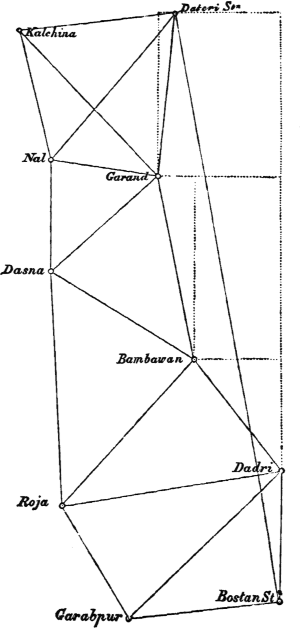
\includegraphics{images/geodesy-ray-tracing.png}
  \caption{In \gls{geodesy}, ray tracing was historically employed to determine the precise telescope angle required to observe a signal from a distant location. In this illustration from~\cite[p.~xix]{Everest1847}, any city serves as either the observation point or the light source, and the various ray paths connecting the two locations demonstrate the correct telescope angle.}
  \labfig{geodesy-ray-tracing}
\end{marginfigure}

The acoustic echoes of one's voice bouncing off the walls of a tunnel provide an intuitive analogy for radio wave propagation. When a \gls{tx} emits radio signals, they interact with the environment---reflecting off buildings, the ground, and other obstacles---creating multiple distinct paths to the \gls{rx}. This phenomenon is known as multipath propagation. Whether applied to sound, light, or radio waves, ray tracing serves as a powerful technique to model and analyze wave behavior as it propagates through complex environments.

\section{History of Ray Tracing}\labsec{history}

Before addressing the technical details of ray tracing and the theory required for its application to radio waves, it is interesting to understand the method's historical context. While the first explicit mention of \enquote{ray tracing} is likely attributable to Sir George Everest in the context of \gls{geodesy} during the mid-19th century~\sidecite{Everest1847}, the concept of using rays as a high-frequency approximation of waves was developed independently across several fields over more than a century.

In optical design, Alexander Eugen Conrady demonstrated in the late 1920s that the aberration of a lens system could be quantified by tracing a finite number of representative rays through successive interfaces~\sidecite{Conrady1929}. This concept---sampling a continuous wavefront with discrete trajectories---enables the solution of optics problems without requiring an exact solution to the wave equation. This computational simplification underpins all subsequent developments in ray tracing.

Beyond glass optics, the notion of a \enquote{ray} was rapidly generalized to other physical media. In electron optics, Klemperer applied similar principles to charged particles moving in smoothly varying electromagnetic fields, replacing piecewise-linear segments with continuously curved trajectories within an inhomogeneous \enquote{refractive index} defined by the potential~\sidecite{Klemperer1939}. In underwater acoustics, Lichte modeled the ocean as a stratified medium with a depth-dependent speed of sound. He utilized ray theory to predict refraction, \emph{shadow zones}\footnote{Referred to elsewhere in the text as \glspl{shadow region}.}, and deep sound channels, foreshadowing later work on long-range sonar and the \gls{sofar} channel~\sidecite{Lichte1919}. This body of work was systematized during World War II by the \gls{ndrc} report on the physics of sound in the sea, which popularized ray diagrams as the standard language for explaining propagation, ducting, and shadowing to sonar operators~\sidecite{NDRC1946}.

Radio physicists developed an equally rich ray theory for the ionosphere. Booker's analysis of wave packets in a doubly refracting plasma clarified that a radio \enquote{ray} should be identified with the trajectory of energy flow (group velocity), which differs from the phase-normal direction in anisotropic media~\sidecite{Booker1938}. Millington provided graphical constructions for such rays in a curved ionosphere, while Haselgrove recast the problem into a Hamiltonian system of differential equations amenable to numerical integration on early digital computers~\sidecite{Millington1954,Haselgrove1955}. Her formulation marked a pivotal transition: the shift from hand-drawn ray sketches to fully algorithmic ray tracing in generic, inhomogeneous media---a pattern that would later reemerge in seismology and computer graphics.

\begin{figure}
  \centering
  \begin{subfigure}[t]{0.48\textwidth}
    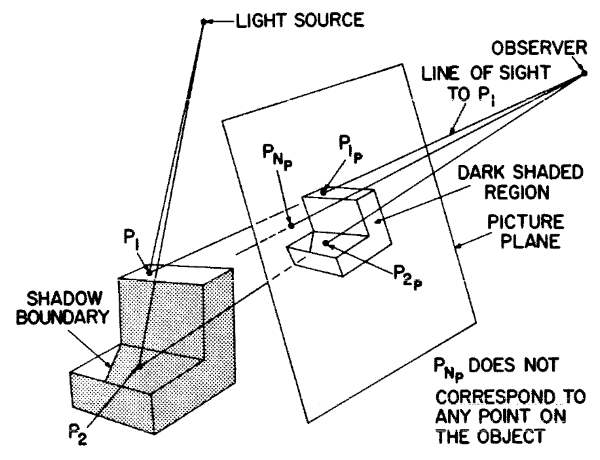
\includegraphics[width=\textwidth]{images/appel-shading.png}
    \caption{Point-by-point shading.}
    \labfig{appel-shading}
  \end{subfigure}
  \hfill
  \begin{subfigure}[t]{0.48\textwidth}
    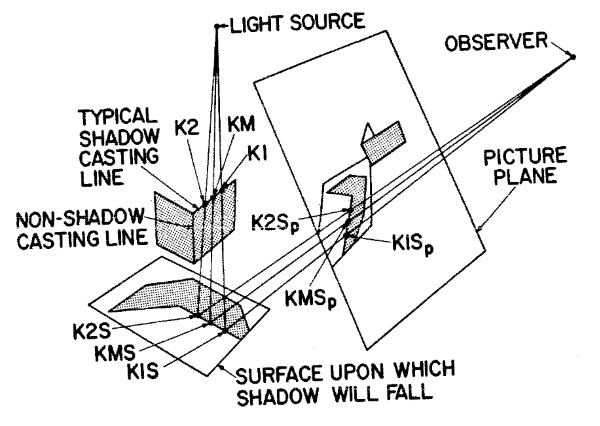
\includegraphics[width=\textwidth]{images/appel-shadows.png}
    \caption{Segment-by-segment outlining of shadows.}
    \labfig{appel-shadows}
  \end{subfigure}
  \caption{Appel's ray tracing methods for computing the shading and shadowing of an object, from~\cite[Fig.~6~\&~7]{Appel1968}.}
  \labfig{appel-ray-tracing}
\end{figure}

In computer graphics, ray tracing emerged in the late 1960s as a mechanism for solving visibility and shading problems. Appel's algorithm cast rays from the viewpoint through each pixel, intersected them with scene geometry, and spawned secondary rays toward light sources to determine if a point was illuminated or shadowed~\sidecite{Appel1968}. Whitted generalized this approach by introducing recursive rays for reflection and refraction, providing a unified framework for specular transport capable of rendering mirror-like and transparent objects with unprecedented realism~\cite{Whitted1980}. This lineage culminated in path tracing and the rendering equation, where rays are interpreted as Monte Carlo samples of an underlying transport integral, conceptually echoing Conrady's finite set of representative rays, albeit in a stochastic setting.

\begin{marginfigure}
  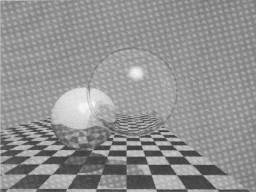
\includegraphics{images/whitted-rendering.png}
  \caption{Example image rendered using Whitted's model, from~\cite[Fig.~7]{Whitted1980}.}
  \labfig{whitted-rendering}
\end{marginfigure}

Around the same time, acoustics researchers began applying similar techniques to develop an accurate theory of sound reverberation. In 1967, Atal and Schroeder presented what was likely the first application of ray tracing to model room acoustics~\sidecite{Atal1967}. Independently, Krokstad, Strøm, and Sørsdal published work on calculating the acoustical room response using ray tracing~\sidecite{Krokstad1968}.

Simultaneously, seismology adopted ray tracing to study the propagation of seismic waves through the Earth's interior. Julian and Gubbins formulated practical \enquote{shooting} and \enquote{bending} schemes to solve the two-point boundary-value problem: finding a ray that connects an earthquake source to a receiver through a heterogeneous velocity field~\sidecite{Julian1977}. Červený and Hron extended this kinematic ray theory to \emph{dynamic} ray tracing, augmenting the path equations with additional differential equations for geometrical spreading and wavefront curvature. This allowed for the prediction of amplitudes in addition to travel times~\sidecite{Cerveny1980}. These developments established ray tracing as the workhorse of seismic tomography and earthquake location.

From the 1980s onward, ray-based methods in electromagnetism began to connect more directly to the propagation problems considered in this book. The \gls{sbr} method combined geometric optics inside complex cavities with a final \gls{po} integration on apertures to estimate the radar cross-sections of electrically large structures~\sidecite{Ling1989}. In terrestrial wireless communications, deterministic ray tracing in urban environments was used to predict path loss and delay spread by modeling buildings as reflective and diffracting obstacles~\sidecite{Schaubach1992}, an approach later surveyed and generalized in comprehensive reviews of radio propagation modeling~\sidecite{Yun2015}.

\begin{figure}[h]
  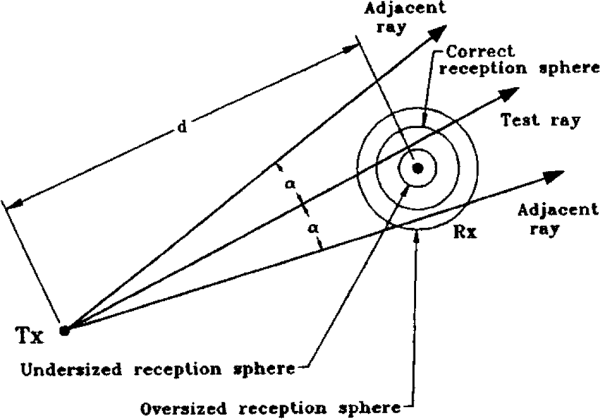
\includegraphics[width=0.75\textwidth]{images/interception-sphere.png}
  \caption{Concept of an interception sphere around the receiver to capture incoming rays from all directions, from~\cite[Fig.~2]{Schaubach1992}.}
  \labfig{interception-sphere}
\end{figure}

In parallel, Keller's \glsxtrfull{gtd} and the subsequent \glsxtrfull{utd} by Kouyoumjian and Pathak extended classical geometric optics by introducing diffracted rays. This provided a consistent high-frequency treatment of shadow boundaries and edge diffraction, which is now standard in high-frequency radio models~\sidecite{Keller1962,Kouyoumjian1974}.

\begin{figure}[h]
  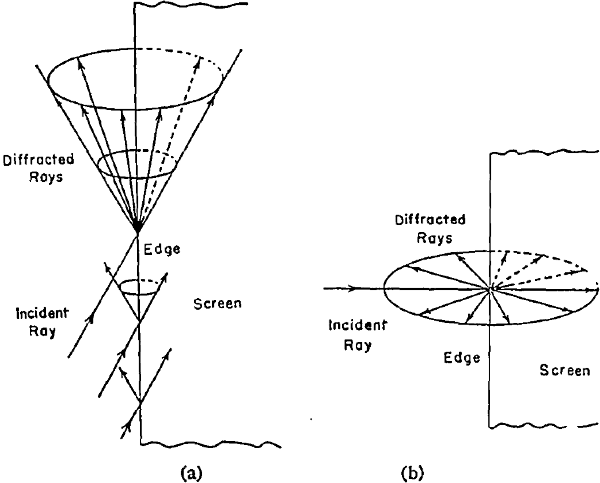
\includegraphics[width=0.75\textwidth]{images/keller-cone-and-plane.png}
  \caption{Keller's cone (a) and plane (b) of diffraction, from~\cite[Fig.~1]{Keller1962}.}
  \labfig{keller-cone-and-plane}
\end{figure}

The turn of the 21st century marked a paradigm shift with the utilization of \glspl{gpu} for general-purpose scientific computing, instead of traditional \glspl{cpu}. In 2002, Purcell \etal demonstrated the first full ray tracing pipeline running on programmable graphics hardware, effectively treating the \gls{gpu} as a stream processor for global illumination rather than just \gls{rasterization}~\sidecite{Purcell2002}. This proof-of-concept evolved rapidly with the advent of compute-unified device architectures (such as NVIDIA CUDA) and dedicated ray tracing engines like NVIDIA OptiX~\sidecite{Parker2010}, which abstracted the complexities of parallel intersection tests and bounding volume hierarchy management.

These advances in computer graphics were rapidly adopted by the radio propagation community to address the heavy computational burden of deterministic channel modeling. By porting algorithms like \gls{sbr} to \glspl{gpu}, researchers achieved orders-of-magnitude speedups compared to traditional \gls{cpu}-based solvers. This leap in performance enabled the simulation of massive numbers of interactions in complex urban environments in near real-time, moving ray tracing from offline analysis to potential online applications. The subsequent integration of dedicated hardware acceleration---such as ray tracing cores in modern consumer \glspl{gpu}---has further cemented this approach, providing the computational throughput necessary for the deep learning integration described below.

Since then, the most recent evolutions of ray tracing have been tightly coupled with machine learning and inverse problems. Differentiable ray tracing, as introduced by Li \etal, enables the fast and convenient computation of gradients for rendered images with respect to geometry, materials, and lighting---even in the presence of discontinuities. This capability effectively transforms ray tracing into a differentiable layer within deep learning pipelines~\sidecite{Li2018}. Furthermore, the emergence of \gls{gpu}-oriented differentiable frameworks such as TensorFlow, PyTorch, or JAX has made it possible to adopt these techniques in more user-friendly and popular programming languages like Python while maintaining high performance through \gls{jit} compilation~\sidecite{TensorFlow2015,PyTorch2024,Jax2018}. Building on these ideas, Sionna~RT and DiffeRT, two open-source Python programs, apply differentiable ray tracing to radio propagation, allowing transmit configurations, antenna orientations, and material parameters to be optimized via gradient-based methods in an end-to-end communication system model~\sidecite{Hoydis2023,Eertmans2025ICMLCNDemo}.

In this sense, the historical trajectories of optics, acoustics, seismology, computer graphics, and electromagnetics converge: the \enquote{ray} becomes a universal computational primitive for high-frequency wave propagation, and its differentiable variant is merely the latest iteration.

\section{The High-Frequency Approximation}\labsec{hf-approximation}

In \refch{propagation}, we discussed the full-wave nature of electromagnetic fields. However, solving the wave equation directly becomes computationally intractable when the environment is large compared to the \gls{wavelength}. Then, through the knife-edge and two-ray models, we introduced solutions to the wave propagation problem that only consider a discrete number of trajectories that we refer to as \emph{ray paths}. In this section, we will provide the theoretical framework that allows us to approximate the wave as a bundle of rays when the frequency is high enough.

\subsection{From Waves to Rays: The Lüneburg-Kline Expansion}

Using the Lüneburg\footnote{While many papers, including Kline's, cite him as Luneberg, the correct spelling is Lüneburg.}-Kline ansatz~\sidecite{Luneburg1944,Kline1951}, we can express the high-frequency electromagnetic fields in a source-free region occupied by isotropic media as an asymptotic power series in inverse powers of frequency $\omega$ as
\begin{align}
  \bsup{E}(\bsup{r}, \omega) &\sim e^{-jk \Psi(\bsup{r})} \sum_{m=0}^{\infty} \frac{\bsup{E}_m(\bsup{r})}{(j\omega)^m},\label{eq:luneberg-kline-e}\\
  \bsup{H}(\bsup{r}, \omega) &\sim e^{-jk \Psi(\bsup{r})} \sum_{m=0}^{\infty} \frac{\bsup{H}_m(\bsup{r})}{(j\omega)^m},\label{eq:luneberg-kline-h}
\end{align}
where $\sim$ indicates an asymptotic equality, $\Psi(\bsup{r})$ is the phase function, and $k = \omega v^{-1}$ is the \gls{wavenumber}.

To derive the fundamental equations of ray optics, we substitute the asymptotic expansions~\eqref{eq:luneberg-kline-e} and~\eqref{eq:luneberg-kline-h} into the source-free Maxwell's equations~\sidecite[][Secs.~2.2.4 and 2.2.5]{McNamara1990}. For the remainder of this section, we will drop the explicit dependency on $\bsup{r}$ for brevity. For instance, considering Faraday's law in the time-harmonic case~\eqref{eq:th-faraday}, and applying the vector identity
\begin{equation}
  \nabla \times (f\bsup{F}) = \nabla f \times \bsup{F} + f \nabla \times \bsup{F},
\end{equation}
with
\begin{equation}
  f = e^{-jk\Psi},
\end{equation}
and
\begin{equation}
  \bsup{F} = \sum\limits_{m=0}^{\infty} \frac{\bsup{E}_m}{(j\omega)^m},
\end{equation}
we obtain
\begin{wideequation}
  e^{-jk\Psi} \sum_{m=0}^{\infty} \left[ \frac{\nabla \times \bsup{E}_m}{(j\omega)^m} - \frac{1}{v} \frac{\nabla \Psi \times \bsup{E}_m}{(j\omega)^{m-1}} \right] = -\mu e^{-jk\Psi} \sum_{m=0}^{\infty} \frac{\bsup{H}_m}{(j\omega)^{m-1}},
\end{wideequation}
where we used the relation $k = \omega v^{-1}$.

At high frequencies, the denominator $\omega^m$ becomes extremely large, so that the terms in the series decrease very rapidly. We can therefore reasonably truncate the series when the exponent is greater than $0$, and simplify the expression, which leads to
\begin{wideequation}\label{eq:luneberg-kline-faraday-truncated}
  \left[ \frac{v^{-1} (\nabla \Psi \times \bsup{E}_0)}{(j\omega)^{-1}} + \frac{v^{-1} (\nabla \Psi \times \bsup{E}_1) - \nabla \times \bsup{E}_0}{(j\omega)^0} \right] = \mu \left[\frac{\bsup{H}_0}{(j\omega)^{-1}} + \frac{\bsup{H}_1}{(j\omega)^0}\right].
\end{wideequation}

Because~\eqref{eq:luneberg-kline-faraday-truncated} must hold for different frequencies, we can equate the left- and right-hand side coefficients of the different powers of $j\omega$. For the leading-order terms, we find
\begin{equation}
  \frac{1}{v}\left(\nabla \Psi \times \bsup{E}_0\right) = \mu \bsup{H}_0.\label{eq:go-faraday}
\end{equation}

A similar procedure applied to the other Maxwell's equations in the time-harmonic case~\eqref{eq:th-ampere_maxwell},~\eqref{eq:th-gauss_elec}, and~\eqref{eq:th-div_mag}, yields three additional relations for the leading-order terms
\begin{align}
  \frac{1}{v}\left(\nabla \Psi \times \bsup{H}_0\right) &= -\epsilon \bsup{E}_0,\label{eq:go-ampere}\\
  \nabla \Psi \cdot \bsup{E}_0 &= 0,\label{eq:E-orthogonality}\\
  \nabla \Psi \cdot \bsup{H}_0 &= 0.\label{eq:H-orthogonality}
\end{align}

Equations~\eqref{eq:E-orthogonality} and~\eqref{eq:H-orthogonality} reveal that the electric and magnetic field vectors are orthogonal to each other and to the direction of propagation $\nabla \Psi$, confirming that high-frequency waves behave locally as uniform \gls{tem} plane waves.

\subsection{The Eikonal Equation}

We can rewrite the first relation~\eqref{eq:go-faraday} using the intrinsic impedance $Z = \sqrt{\tfrac{\mu}{\epsilon}} = \mu v$ to obtain
\begin{equation}
  \bsup{H}_0 = \frac{1}{Z} (\nabla \Psi \times \bsup{E}_0).
\end{equation}

Substituting this into~\eqref{eq:go-ampere} and applying the vector triple product identity gives
\begin{equation}
  (\nabla \Psi \cdot \bsup{E}_0) \nabla \Psi - |\nabla \Psi|^2 \bsup{E}_0 = -\bsup{E}_0.
\end{equation}

Since $\nabla \Psi \cdot \bsup{E}_0 = 0$ from~\eqref{eq:E-orthogonality}, the previous equation simplifies directly to what is called the \emph{eikonal equation}
\begin{equation}\label{eq:eikonal}
  |\nabla \Psi|^2 = 1.
\end{equation}

As a consequence, the phase function $\Psi(\bsup{r})$ is sometimes referred to as the \emph{eikonal function}. In this normalization, $\Psi$ has the dimension of length and can be interpreted as an optical path-length coordinate. In homogeneous media, it grows linearly along each ray trajectory.

\subsection{The Transport Equations}

While the eikonal equation determines the phase variation along the propagation path of high-frequency fields, the amplitude variation along this path is governed by the \emph{transport equations}. These are obtained by substituting the Lüneburg-Kline expansion for the electric field~\eqref{eq:luneberg-kline-e} into the vector Helmholtz equation~\eqref{eq:helmholtz}. After differentiating and grouping the terms by powers of $j\omega$, we obtain
\begin{wideequation}
  e^{-jk\Psi} \sum_{m=0}^{\infty} \left[ \frac{(1 - |\nabla \Psi|^2) \bsup{E}_m}{v(j\omega)^{m-2}} - \frac{\bsup{E}_m \nabla^2 \Psi + 2(\nabla \Psi \cdot \nabla)\bsup{E}_m}{v(j\omega)^{m-1}} + \frac{\nabla^2 \bsup{E}_m}{(j\omega)^m} \right] = 0.
\end{wideequation}
% NOTE: the first term (1 + |Psi|^2) E_m is not equal to (1 + |Psi|^2 E_m from the book (Eq. 2.25), but the one from the McNamara book doesn't lead to the eikonal equation, so I think there is a typo in the McNamara book.

Again, we can equate the coefficients of the different powers of $j\omega$ by grouping terms of equal magnitude in inverse powers of frequency. For the $(j\omega)^2$ coefficients, we re-obtain the eikonal equation. In the case of the coefficients of $(j\omega)^1$, we obtain the \emph{zeroth-order transport equation}
\begin{equation}\label{eq:zero-order-transport}
  2 (\nabla \Psi \cdot \nabla) \bsup{E}_0 + (\nabla^2 \Psi) \bsup{E}_0 = 0.
\end{equation}

This equation enforces the conservation of energy flux. As a wave propagates, the term $\nabla^2 \Psi$ acts as a measure of the wavefront's curvature: positive values correspond to local divergence (amplitude decay), while negative values correspond to convergence (amplitude growth). In the locally planar limit, $\nabla^2 \Psi \to 0$, so amplitude changes are driven only by higher-order effects.

Equating the $(j\omega)^0$ terms leaves only one remaining relation
\begin{equation}
  \nabla^2 \bsup{E}_0 = 0.
\end{equation}

Finally, the \emph{higher-order transport equations} are obtained by equating the coefficients of the remaining powers of $j\omega$, i.e.,
\begin{equation}
  2 (\nabla \Psi \cdot \nabla) \bsup{E}_m + (\nabla^2 \Psi) \bsup{E}_m = -v \nabla^2 \bsup{E}_{m-1},
\end{equation}
with $m\ge 1$, but they are not used in the high-frequency approximation.

\subsection{\glsentryshort{go} Ray Trajectories Follow Straight Lines}

As motivated earlier, the higher-order terms in the asymptotic expansions~\eqref{eq:luneberg-kline-e} and~\eqref{eq:luneberg-kline-h} can be neglected in the high-frequency approximation. The only remaining terms are the lowest ones: $\bsup{E}_0$ and $\bsup{H}_0$. Those are called the \gls{go} field terms
\begin{align}
  \bsup{E}(\bsup{r}, \omega) &\underset{\omega \to \infty}{\sim} \bsup{E}_0(\bsup{r}) e^{-jk \Psi(\bsup{r})},\label{eq:go-e-field}\\
  \bsup{H}(\bsup{r}, \omega) &\underset{\omega \to \infty}{\sim} \bsup{H}_0(\bsup{r}) e^{-jk \Psi(\bsup{r})}.\label{eq:go-h-field}
\end{align}

By reusing what we have derived in the previous sections, we can compute the Poynting vector
\begin{align}
  \bsup{S} &= \bsup{E}\times\bsup{H}^*,\\
  &= \frac{1}{Z} \bsup{E}_0 \times \bsup{H}_0^*,\\
  &= \frac{1}{Z} (\bsup{E}_0 \cdot \bsup{E}_0^*) \nabla \Psi,\\
  &= \frac{1}{Z} |\bsup{E}_0|^2 \nabla \Psi,
\end{align}
which indicates that the power flows along the direction of propagation $\nabla \Psi$.

Moreover, the eikonal equation~\eqref{eq:eikonal} imposes that $|\nabla \Psi| = 1$, which means that the direction of the Poynting vector $\uvec{s}$ is exactly equal to $\nabla \Psi$. We call this the \emph{ray direction}. Since $\uvec{s}$ is a unit vector, \gls{go} rays can be understood as curves everywhere tangent to this direction, representing the paths along which electromagnetic energy propagates.

\begin{figure}
  \centering
  \inputtikz{ray-tube}
  \caption{Narrow ray tube, reproduced from~\cite[Fig.~2.2]{McNamara1990}.}
  \labfig{ray-tube}
\end{figure}

A fundamental property of \gls{go} is that energy transport occurs exclusively along ray trajectories---there is no transverse energy flow perpendicular to a ray. This leads naturally to the concept of a \emph{ray tube}: a bundle of neighboring rays surrounding a central reference ray, as illustrated in \reffig{ray-tube}. Because the boundary of such a tube is constructed from the trajectories of adjacent rays, and because energy cannot cross these boundaries, the electromagnetic power passing through any cross-section of a given ray tube remains constant in the absence of absorption or scattering. This power conservation principle is central to understanding how field amplitudes evolve as wavefronts expand or contract.

From the orthogonality of $\bsup{E}_0$ and $\bsup{H}_0$ with respect to $\nabla \Psi$, we can deduce that the \gls{go} fields act locally as plane waves.

Now that we have established this, we still are missing information about the ray trajectory, polarization, amplitude and phase of the wave as it propagates.

\subsubsection{Ray Trajectories}\labsec{ray-trajectories}

\begin{figure}
  \centering
  \inputtikz{ray-coordinate-system}
  \caption{Ray coordinate system, reproduced from~\cite[Fig.~2.3]{McNamara1990}.}
  \labfig{ray-coordinate-system}
\end{figure}

For the trajectory, we express the position vector $\bsup{r}$ as a function of a single coordinate $s$ measured along the propagation direction $\uvec{s}$, as shown in \reffig{ray-coordinate-system}. An infinitesimal increment in the position vector $\mathrm{d}\bsup{r}$ is related to the infinitesimal increment in $s$ through the relation
\begin{equation}
  \mathrm{d}\bsup{r} = \uvec{s}\mathrm{d}s.
\end{equation}

Then, we can rewrite the eikonal equation~\eqref{eq:eikonal} as
\begin{equation}
  \frac{\mathrm{d}\Psi}{\mathrm{d}s} = 1,
\end{equation}
and the zeroth-order transport equation~\eqref{eq:zero-order-transport} as
\begin{equation}
  2 \frac{\mathrm{d}\bsup{E}_0}{\mathrm{d}s} + (\nabla^2\Psi) \bsup{E}_0 = 0.
\end{equation}

For the ray trajectory, differentiating the relation $\tfrac{\mathrm{d}\bsup{r}}{\mathrm{d}s} = \nabla\Psi$ with respect to $s$ yields
\begin{equation}
  \frac{\mathrm{d}^2\bsup{r}}{\mathrm{d}s^2} = \frac{\mathrm{d}}{\mathrm{d}s}(\nabla\Psi) = (\uvec{s}\cdot\nabla)\nabla\Psi = (\nabla\Psi\cdot\nabla)\nabla\Psi.
\end{equation}

Using the vector identity $(\nabla\Psi\cdot\nabla)\nabla\Psi = \tfrac{1}{2}\nabla(|\nabla\Psi|^2)$ along with the eikonal equation~\eqref{eq:eikonal}, we obtain the second-order differential equation,
\begin{equation}
  \frac{\mathrm{d}^2\bsup{r}}{\mathrm{d}s^2} = 0,
\end{equation}
which has a solution in the form of a straight line
\begin{equation}
  \bsup{r}(s) = \bsup{A} + s \bsup{B},
\end{equation}
where $\bsup{A}$ and $\bsup{B}$ are constant vectors.

Although we have demonstrated that the trajectories of \gls{go} fields follow straight lines in homogeneous media, it is important to note that \textbf{this is not true in inhomogeneous media}, where the ray trajectories are curved. While it is not trivial to solve for the exact ray trajectories in inhomogeneous media, it is possible to do so in piecewise homogeneous media, which is the case in most practical scenarios. In these media, rays travel in straight lines within homogeneous regions but bend at interfaces according to Snell's law.

Lastly, it is essential to highlight that ray tracing algorithms almost always assume that ray trajectories are linear. Consequently, for the remainder of this book, when we refer to ray trajectories, we are referring to straight line segments.

\subsubsection{Polarization}

As discussed in \refch{propagation}, we can express the electric and magnetic fields of a locally plane wave as combinations of two orthogonal polarizations. In the non-restrictive case of a single polarization direction for both fields, which we denote as the unit vectors $\uvec{e}$ and $\uvec{h}$ for the electric and magnetic fields, respectively, we can write
\begin{equation}
  \uvec{e} = \frac{\bsup{E}_0}{|\bsup{E}_0|}, \quad \text{and} \quad \uvec{h} = \frac{\bsup{H}_0}{|\bsup{H}_0|}.
\end{equation}

From the properties established in the previous sections, these unit vectors are orthogonal to the ray direction $\uvec{s}$, yielding
\begin{equation}
  \uvec{e} \cdot \uvec{s} = 0, \quad \text{and} \quad \uvec{h} = \uvec{s} \times \uvec{e}.
\end{equation}

To determine how the polarization behaves as the wave propagates, we evaluate its change along the ray trajectory by examining the derivative $\tfrac{\mathrm{d}\uvec{e}}{\mathrm{d}s}$. Using the definition of $\uvec{e}$ along with the zeroth-order transport equation~\eqref{eq:zero-order-transport}, we can algebraically deduce that this derivative vanishes
\begin{equation}
  \frac{\mathrm{d}\uvec{e}}{\mathrm{d}s} = 0.
\end{equation}

This result demonstrates that the polarization vector $\uvec{e}$ remains constant as the ray propagates through homogeneous regions. Consequently, once the polarization is initialized at a reference point, it is perfectly defined along the entirety of the ray path until it interacts with an object. This property simplifies ray tracing, allowing us to only consider polarization changes during discrete interactions (like reflections, transmissions, or diffractions).

For more complex fields exhibiting circular or elliptical polarizations, linearity allows us to decompose the field into two orthogonal linear components, track their constant polarization directions independently along the ray paths, and recombine them to find the total state.

\subsubsection{Phase}

The phase variation of the \gls{go} field along a ray trajectory is governed by the eikonal equation~\eqref{eq:eikonal}, taking the form $|\nabla \Psi| = 1$. In a homogeneous medium, where rays are straight lines and orthogonal to the equiphase surfaces, the incremental phase change $\mathrm{d}\Psi$ over a small distance $\mathrm{d}s$ is simply
\begin{equation}
  \mathrm{d}\Psi = |\nabla \Psi| \mathrm{d}s = \mathrm{d}s.
\end{equation}

Integrating this relation along the ray path from a reference origin $s_0$ to an arbitrary distance $s$ yields
\begin{equation}
  \Psi(s) - \Psi(s_0) = s - s_0.
\end{equation}

By adopting the convention that the reference point is placed at $s_0 = 0$, the phase function evolution simplifies to
\begin{equation}
  \Psi(s) = \Psi(0) + s.
\end{equation}

Consequently, the exponential phase term describing the spatial oscillation of the field along the ray reduces to
\begin{equation}
  e^{-jk\Psi(s)} = e^{-jk\Psi(0)} e^{-jks}.
\end{equation}

\subsubsection{Amplitude}

The final element required to fully define the \gls{go} field behavior is the amplitude continuation function. To obtain this, we must solve the zeroth-order transport equation~\eqref{eq:zero-order-transport}. This differential equation can be integrated with respect to $s$ from the reference point $s=0$ to yield
\begin{equation}\label{eq:amplitude-integral}
  \bsup{E}_0(s) = \bsup{E}_0(0) \exp\left[ -\frac{1}{2} \int\limits_{0}^{s} \nabla^2 \Psi \, \mathrm{d}s' \right].
\end{equation}

To make~\eqref{eq:amplitude-integral} practically useful, we must evaluate the Laplacian of the phase, $\nabla^2 \Psi$, which relates to the curvature of the wavefront. First, we define an \emph{astigmatic ray tube} to be a narrow bundle of rays centered around a central ray, as illustrated in \reffig{ray-tube}. At the reference wavefront $\Psi(0)$, the tube has two principal radii of curvature, $\rho_1$ and $\rho_2$. As the wave propagates a distance $s$ along the central ray to reach surface $\Psi(s)$, these principal radii expand to $\rho_1 + s$ and $\rho_2 + s$. This is illustrated in \reffig{ray-tube-diverging}.

\begin{figure*}
  \centering
  \inputtikz{ray-tube-diverging}
  \caption{Diverging astigmatic ray tube, reproduced from~\cite[Fig.~2.4]{McNamara1990}.}
  \labfig{ray-tube-diverging}
\end{figure*}

The ratio of the physical cross-sectional area of the ray tube at distance $s$ to its area at $s=0$ can be connected to the divergence of the power density vector. Through the divergence theorem, this leads to the intensity law (or power conservation along the ray tube), allowing us to rewrite the exponential term analytically as the square root of the ratio of the ray tube areas. Thus, the field amplitude evolves as
\begin{equation}
  \bsup{E}_0(s) = \bsup{E}_0(0) \sqrt{\frac{\rho_1 \rho_2}{(\rho_1 + s)(\rho_2 + s)}}.
\end{equation}

Combining the amplitude, phase, and polarization components, the complete and final expression for the \gls{go} electric field at a distance $s$ from a reference point is
\begin{equation}\label{eq:go-continuation}
  \bsup{E}(s) = \bsup{E}(0) \sqrt{\frac{\rho_1 \rho_2}{(\rho_1 + s)(\rho_2 + s)}} e^{-jks},
\end{equation}
where we have incorporated the initial phase $e^{-jk\Psi(0)}$ into the complex reference field $\bsup{E}(0)$.

Equation~\eqref{eq:go-continuation} represents the \emph{ray optical continuation}. Given the initial complex vector field $\bsup{E}(0)$ and the wavefront's principal radii of curvature $\rho_1$ and $\rho_2$ at a known point, we can compute the precise characteristics of the \gls{go} field at any subsequent point along the ray trajectory. The square-root term,
\begin{equation}\label{eq:spreading-factor}
  A(s) = \sqrt{\frac{\rho_1 \rho_2}{(\rho_1 + s)(\rho_2 + s)}},
\end{equation}
is called the \emph{spreading factor}, and it accounts for the divergence or convergence of the ray tube as the wavefront propagates. For plane waves ($\rho_1,\rho_2 \to \infty$), the spreading factor approaches unity, while for curved wavefronts it modulates the amplitude decay (or growth, if the wave converges).

This analytical simplicity is a key strength of ray tracing, although the formulation does break down when the ray tube converges precisely to a line or point ($\rho_1 + s = 0$ or $\rho_2 + s = 0$). Such locations are known as \emph{caustics}, and at these points, equation~\eqref{eq:go-continuation} incorrectly predicts an infinite field magnitude. Modeling the true bounded fields near caustics requires more advanced techniques that fall beyond the scope of simple \gls{go}.

Three special cases of wavefront curvature are worth noting: planar wavefronts, cylindrical wavefronts, and spherical wavefronts. All of them are solutions to the eikonal equation~\eqref{eq:eikonal}.

\paragraph{Plane waves}

For a plane wave, both principal radii of curvature approach infinity ($\rho_1 \to \infty$ and $\rho_2 \to \infty$), indicating that the wavefront surfaces are perfectly flat and parallel. Substituting these limits into~\eqref{eq:go-continuation}, the spreading factor reduces to unity, yielding
\begin{equation}
  \bsup{E}(s) = \bsup{E}(0) e^{-jks}.
\end{equation}

This expression shows that plane waves propagate without amplitude decay due to spreading---only the phase advances linearly with distance. This idealization is often used to approximate fields in the \glshyph{far field} region of a source, where the wavefront curvature becomes negligible over the observation region.

\paragraph{Cylindrical waves}

A cylindrical wave arises when one principal radius of curvature is finite while the other approaches infinity. Without loss of generality, let $\rho_1 \to \infty$ and $\rho_2 = \rho$. This corresponds to a wavefront that is flat in one transverse direction but curved in the other, such as the field radiated by an infinite line source. Applying these conditions to~\eqref{eq:go-continuation} gives
\begin{equation}
  \bsup{E}(s) = \bsup{E}(0) \sqrt{\frac{\rho}{\rho + s}} e^{-jks}.
\end{equation}

The amplitude decays proportionally to $\tfrac{1}{\sqrt{s}}$ as $s$ becomes large compared to $\rho$, reflecting the one-dimensional spreading of energy in the curved direction.

\paragraph{Spherical waves}

When both principal radii of curvature are equal and finite ($\rho_1 = \rho_2 = \rho$), the wavefront is spherical, characteristic of radiation from a point source. Equation~\eqref{eq:go-continuation} simplifies to
\begin{equation}
  \bsup{E}(s) = \bsup{E}(0) \frac{\rho}{\rho + s} e^{-jks}.
\end{equation}

For large distances where $s \gg \rho$, this reduces to the familiar $\tfrac{1}{s}$ amplitude decay, corresponding to the inverse-distance law for spherical wave propagation. This is the most common wavefront geometry encountered in practical antenna radiation and point-source scattering problems.

\subsection{Fermat's Principle}\labsec{fermat-principle}

An alternative and powerful formulation for determining ray trajectories is provided by \emph{Fermat's principle}, which states that the path taken by a ray between two points is such that the \emph{optical path length} is stationary (typically a minimum, but more generally an extremum). The optical path length $L$ along a trajectory from point $\bsup{A}$ to point $\bsup{B}$ is defined as
\begin{equation}
  L = \int\limits_{\bsup{A}}^{\bsup{B}} n(s)\,\mathrm{d}s,
\end{equation}
where $n(s)$ is the refractive index of the medium and the integral is taken along the ray path.

In a homogeneous medium with constant $n$, this reduces to simply the geometric distance, and Fermat's principle confirms that rays travel in straight lines. However, the true utility of Fermat's principle emerges when rays interact with boundaries or propagate through inhomogeneous media. At interfaces, the principle directly leads to laws of reflection and refraction, as derived by Snell, without requiring explicit solution of the transport equations.

Fermat's principle provides a practical advantage to ray tracing algorithms. Rather than solving differential equations for ray trajectories, the problem can be redefined as an optimization problem: finding the path that extremizes optical length. This variational approach is extremely valuable in scenarios involving reflections, refractions, and diffractions at surfaces because the interaction points and ray directions can be determined by enforcing the stationarity condition. This geometric interpretation is fundamental to many efficient ray tracing techniques, the most important of which will be introduced in \refch{path-tracing}, and it provides intuitive insight into the physical behavior of high-frequency wave propagation.

\subsection{\texorpdfstring{\glsentrytitlecase{go}{long}}{Geometrical Optics} versus \texorpdfstring{\glsentrytitlecase{po}{long}}{Physical Optics}}\label{sec:go_vs_po}

At this stage, we should clearly distinguish two asymptotic frameworks that apply to high frequencies: \glsxtrfull{go} and \glsxtrfull{po}. Both operate in the short-\gls{wavelength} regime, but they model wave--object interactions differently.

\gls{go} is the framework developed in the previous sections. It represents propagation through ray trajectories governed by the eikonal equation, with amplitude and phase continued by the transport equations and the spreading factor. Interactions are treated locally through geometric laws (e.g., reflection or refraction), which makes the method computationally efficient and well suited to large deterministic channel simulations. As we will see later in this chapter, its main limitation is also geometric: classical \gls{go} predicts discontinuous fields at shadow boundaries and no field in \glspl{shadow region}.

\gls{po}, in contrast, is a surface-current formulation. The incident field (often obtained from a \gls{go} construction) is first used to approximate equivalent electric and magnetic currents on illuminated parts of a scatterer, and the scattered field is then evaluated through surface integration of those currents. This description better captures finite-surface scattering and naturally yields continuous transitions near shadow boundaries, but at a much higher computational cost because each interaction requires evaluating surface integrals.

For the remainder of this book, we adopt a \gls{go}-based ray tracing model and account for its shadow-boundary deficiencies with \gls{utd}. The purpose of this subsection is therefore not to develop \gls{po}, but to clarify terminology and scope before introducing reflection and diffraction models in the next sections.

\section{Antenna Modeling in Ray Tracing}\labsec{antenna}

In \refch{propagation}, we introduced the fundamental properties of antennas, including their radiation patterns, directivity, and gain. However, a complete electromagnetic model of an antenna involves solving Maxwell's equations in the \glshyph{near field} region, which is computationally prohibitive for large-scale ray tracing simulations. Fortunately, for typical wireless communication scenarios, the interactions between transmitters and receivers occur in the \glshyph{far field} region, where a significantly simplified model can be employed. This section describes how antennas are modeled in ray tracing frameworks through \glshyph{far field} approximations.

\subsection{Transmitting Antenna}

In the \glshyph{far field} region of an antenna radiating in \gls{free space}, the electric field can be accurately represented as a \emph{spherical wave} emanating from the antenna's phase center. At a point in space defined by spherical coordinates $(r, \theta, \varphi)$, where $r$ is the radial distance, $\theta$ is the polar angle, and $\varphi$ is the azimuth angle, the electric field phasor of the radiated wave takes the form
\begin{equation}\labeq{antenna-far-field}
  \bsup{E}(r, \theta, \varphi) = \bsup{E}_0(\theta, \varphi) \frac{e^{-jkr}}{r},
\end{equation}
where $\bsup{E}_0(\theta, \varphi)$ is the complex vector amplitude that depends on the direction of observation but not on the distance. This $\tfrac{1}{r}$ decay reflects the spherical spreading of energy as discussed in the previous section.

To make this expression practical for ray tracing, we introduce the \emph{normalized complex antenna field pattern} $\bsup{F}(\theta, \varphi)$, which characterizes the directional radiation properties of the antenna. According to IEEE Std 145, a radiation pattern describes the spatial distribution of a physical quantity (such as field strength or power density) that characterizes the electromagnetic field generated by an antenna. In particular, a field pattern is defined for a specific component of the electric field (e.g., the $\theta$ or $\varphi$ polarization component) and is normalized to its maximum magnitude. To capture the full polarimetric vector nature, we define the normalized complex field pattern vector $\bsup{F}(\theta, \varphi)$ through its components in the spherical basis as
\begin{equation}
  \bsup{F}(\theta, \varphi) = F_\theta(\theta, \varphi) \uvec{\theta} + F_\varphi(\theta, \varphi) \uvec{\varphi},
\end{equation}
where each component pattern is normalized by the maximum magnitude of the total electric field in the \gls{far field}, i.e.,
\begin{wideequation}
  F_\theta(\theta, \varphi) = \frac{E_{0,\theta}(\theta, \varphi)}{\max_{\theta',\varphi'} \|\bsup{E}_0(\theta', \varphi')\|}, \quad F_\varphi(\theta, \varphi) = \frac{E_{0,\varphi}(\theta, \varphi)}{\max_{\theta',\varphi'} \|\bsup{E}_0(\theta', \varphi')\|}.
\end{wideequation}

By this construction, the maximum magnitude of the normalized complex vector field pattern satisfies
\begin{equation}
  \max_{\theta, \varphi} \|\bsup{F}(\theta, \varphi)\| = 1,
\end{equation}
where $F_\theta$ and $F_\varphi$ are complex-valued functions capturing both the amplitude and phase variation of the respective polarization components.
Because the field pattern is defined using the field envelope $\bsup{E}_0$ rather than the full spherical wave $\bsup{E}(r,\theta,\varphi)$, the radial factor $\tfrac{1}{r}$ is factored out.

The time-averaged Poynting vector for such a spherical wave, which represents the power density per unit area, is given by
\begin{equation}
  \bsup{S}_{\text{avg}}(r, \theta, \varphi) = \frac{1}{2Z_0} \|\bsup{E}(r, \theta, \varphi)\|^2 \uvec{r},
\end{equation}
where $\uvec{r}$ is the radial unit vector.

To describe the angular distribution of radiated power independently of distance, we define the \emph{radiation intensity} $U(\theta, \varphi)$ as the power radiated per unit solid angle. It is obtained by multiplying the radial power density by the square of the distance, i.e.,
\begin{equation}
  U(\theta, \varphi) = r^2 \|\bsup{S}_{\text{avg}}(r, \theta, \varphi)\| = \frac{1}{2Z_0} \|\bsup{E}_0(\theta, \varphi)\|^2.
\end{equation}
Since the time-averaged power density $\|\bsup{S}_{\text{avg}}\|$ decays as $\tfrac{1}{r^2}$ in the \gls{far field} due to the spherical spreading of the electric field magnitude (proportional to $\tfrac{1}{r}$), the multiplication by $r^2$ cancels this distance dependence, leaving $U(\theta, \varphi)$ as a purely angular quantity.

Using the same notation as in the previous chapter, we can find the expression for the directivity $D(\theta, \varphi)$ of a transmitting antenna, which compares its radiation intensity to that of an isotropic radiator, given by
\begin{equation}\labeq{antenna-directivity}
  D(\theta, \varphi) = \frac{U(\theta, \varphi)}{\frac{1}{4\pi}\int_{0}^{2\pi}\int_{0}^{\pi} U(\theta', \varphi') \sin\theta' \, \mathrm{d}\theta' \, \mathrm{d}\varphi'}.
\end{equation}

The gain $G(\theta, \varphi)$ of the transmitting antenna is related to directivity by its radiation efficiency $\eta_{\text{rad}}$. Directivity is purely angular and lossless by construction, whereas gain additionally accounts for ohmic and mismatch losses; the two quantities coincide only when $\eta_{\text{rad}} = 1$. Assuming an ideal, lossless antenna, the total radiated power equals the net power captured by the antenna from the connected transmitter, denoted as $P_t$, and the gain is given by
\begin{align}\labeq{antenna-gain}
  G(\theta, \varphi) &= \frac{U(\theta, \varphi)}{\frac{P_t}{4\pi}} = \frac{2\pi}{Z_0 P_t} \|\bsup{E}_0(\theta, \varphi)\|^2.
\end{align}

The maximum gain of the transmitting antenna is denoted as
\begin{equation}
  G_t \eqdef \max_{\theta, \varphi} G(\theta, \varphi).
\end{equation}

Because $G(\theta, \varphi)$ is proportional to $\|\bsup{E}_0(\theta, \varphi)\|^2$, the normalized field pattern is related to the gain by $G(\theta, \varphi) = G_t \|\bsup{F}(\theta, \varphi)\|^2$. Therefore, we can express the complex amplitude as
\begin{equation}
  \bsup{E}_0(\theta, \varphi) = \sqrt{\frac{P_t G_t Z_0}{2\pi}} \bsup{F}(\theta, \varphi).
\end{equation}

By combining these expressions, we obtain the electric \gls{far field} of a transmitting antenna as a function of the transmit power, maximum gain, and normalized field pattern, given by
\begin{equation}\labeq{transmit-field}
  \bsup{E}_{t}(r, \theta_{t}, \varphi_{t}) = \sqrt{\frac{P_{t} G_{t} Z_0}{2\pi}} \frac{e^{-jkr}}{r} \bsup{F}_{t}(\theta_{t}, \varphi_{t}),
\end{equation}
where $\theta_{t}$ and $\varphi_{t}$ are the angles defining the direction of the ray emanating from the transmitting antenna.

\subsection{Receiving Antenna}

While the transmitting antenna radiates a spherical wave, the receiving antenna typically observes an \emph{incoming plane wave} $\bsup{E}_{r}$ arriving from a specific direction $(\theta_{r}, \varphi_{r})$, defined in the local spherical coordinate system of the receiver. This is because, by reciprocity, the field that has propagated over large distances and potentially undergone multiple interactions appears locally planar at the receiving antenna location. The Poynting vector of this incoming wave is
\begin{equation}
  \bsup{S}_{r} = -\frac{1}{2Z_0} \|\bsup{E}_{r}\|^2 \uvec{r}(\theta_{r}, \varphi_{r}),
\end{equation}
where the negative sign indicates power flow toward the receiving antenna.

The antenna aperture (or effective area) $A_{e,r}$ of the receiving antenna characterizes its ability to extract power from an incident plane wave. For an antenna with gain $G_{r}$, this aperture is related to the \gls{wavelength} by
\begin{equation}\labeq{effective-area}
  A_{e,r}(\theta_{r}, \varphi_{r}) = G_{r}(\theta_{r}, \varphi_{r}) \frac{\lambda^2}{4\pi},
\end{equation}
where $\lambda = \tfrac{2\pi}{k}$ is the \gls{wavelength}. For perfect polarization matching and optimal antenna orientation toward the incoming wave direction, the maximum available received power $P_{r}$ is given by
\begin{equation}
  P_{r} = A_{e,r} \|\bsup{S}_{r}\| = G_{r} \frac{\lambda^2}{4\pi} \frac{\|\bsup{E}_{r}\|^2}{2Z_0}.
\end{equation}

However, in general, the polarization of the incident wave may not align with the receiving antenna's polarization preference, and the wave may arrive from a direction where the antenna gain is not maximal. To account for these effects, we express the received power in terms of the receiving antenna's normalized complex field pattern $\bsup{F}_{r}(\theta_{r}, \varphi_{r})$ and its maximum gain $G_r$. The polarization mismatch is quantified by the polarization efficiency (or polarization mismatch factor) $\eta_{\text{pol}}$, which is the squared magnitude of the inner product between the unit polarization vector representing the antenna's receiving polarization state
\begin{equation}
  \uvec{\rho}_r = \frac{\bsup{F}_r^*(\theta_r, \varphi_r)}{\|\bsup{F}_r(\theta_r, \varphi_r)\|},
\end{equation}
and the unit polarization vector of the incident wave
\begin{equation}\uvec{\rho}_i = \frac{\bsup{E}_r}{\|\bsup{E}_r\|},
\end{equation}
given by
\begin{equation}
  \eta_{\text{pol}} = \left| \uvec{\rho}_r \cdot \uvec{\rho}_i \right|^2 = \left| \frac{\bsup{F}_{r}^{*}(\theta_{r}, \varphi_{r}) \bsup{E}_{r}}{\|\bsup{F}_{r}(\theta_{r}, \varphi_{r})\| \|\bsup{E}_{r}\|} \right|^2,
\end{equation}
where the superscript $*$ denotes the Hermitian transpose (conjugate transpose). Combining this mismatch factor with the directional effective area
\begin{equation}
  A_{e,r}(\theta_r, \varphi_r) = G_r \|\bsup{F}_r(\theta_r, \varphi_r)\|^2 \frac{\lambda^2}{4\pi},
\end{equation}
and the incident power density
\begin{equation}
  \|\bsup{S}_r\| = \frac{\|\bsup{E}_r\|^2}{2Z_0},
\end{equation}
the received power becomes
\begin{wideequation}\labeq{received-power-pattern}
  P_{r} = A_{e,r}(\theta_r, \varphi_r) \|\bsup{S}_r\| \eta_{\text{pol}} = G_r \|\bsup{F}_r(\theta_r, \varphi_r)\|^2 \frac{\lambda^2}{4\pi} \frac{\|\bsup{E}_{r}\|^2}{2Z_0} \left| \frac{\bsup{F}_{r}^{*}(\theta_{r}, \varphi_{r}) \bsup{E}_{r}}{\|\bsup{F}_{r}(\theta_{r}, \varphi_{r})\| \|\bsup{E}_{r}\|} \right|^2.
\end{wideequation}

Since the norms $\|\bsup{F}_r(\theta_r, \varphi_r)\|^2$ and $\|\bsup{E}_r\|^2$ in the numerator and denominator cancel out, this simplifies to the compact received power formula
\begin{equation}
  P_{r} = G_{r} \frac{\lambda^2}{8\pi Z_0} \left| \bsup{F}_{r}^{*}(\theta_{r}, \varphi_{r}) \bsup{E}_{r} \right|^2.
\end{equation}

The inner product term $\bsup{F}_{r}^{*} \bsup{E}_{r}$ naturally accounts for polarization mismatch---if the incident field is orthogonal to the antenna pattern (e.g., a horizontally polarized wave incident on a vertically polarized antenna), the received power vanishes.

The transmitting and receiving antenna models thus define the boundary conditions of a ray-based channel: they determine how fields are launched into the environment and how arriving fields are projected at the receiver. However, as discussed in \refch{propagation}, propagation through realistic environments involves boundary interactions (reflection, transmission, diffraction, etc.) that modify polarization in addition to amplitude and phase. The next ingredient is therefore a compact formalism to propagate polarization through these interactions without repeatedly switching to full vector-field algebra.

\section{Introduction to Jones Calculus}\labsec{jones-calculus}

The propagation and scattering of electromagnetic waves in ray tracing require careful tracking of the polarization state as a field interacts with various objects in the environment. In \refch{propagation}, polarization was introduced as the superposition of two orthogonal transverse components, using the $(\perp,\parallel)$ notation relative to the plane of incidence. We now formalize that idea algebraically. A compact tool for this purpose is \emph{Jones calculus}, originally introduced by R. Clark Jones for polarized light~\sidecite{Jones1941}. Although developed in optics, the same complex two-component formalism applies directly to monochromatic electromagnetic waves in radio propagation: the field is represented in a local transverse basis, and each interaction is modeled as a $2\times2$ complex matrix acting on that vector.

\subsection{Jones Vectors}

Consider a monochromatic plane wave oscillating in a plane perpendicular to its direction of propagation. The complex electric field of this wave can be expressed as a superposition of two orthogonal polarization components. At any point in space, we can decompose this field into components in a local basis; for interactions with surfaces, it is conventionally chosen as the plane of incidence and its perpendicular direction.

Let $\uvec{e}_{\perp}$ and $\uvec{e}_{\parallel}$ denote orthonormal basis vectors perpendicular and parallel to the plane of incidence, respectively. The complex electric field $\bsup{E}$ can then be written as
\begin{equation}
  \bsup{E} = E_{\perp} \uvec{e}_{\perp} + E_{\parallel} \uvec{e}_{\parallel},
\end{equation}
where $E_{\perp}$ and $E_{\parallel}$ are complex amplitudes representing the field components. The \emph{Jones vector} is the compact representation of this field in the local basis
\begin{equation}\label{eq:jones-vector}
  \bsup{e} =
  \begin{bmatrix}
    E_{\perp} \\
    E_{\parallel}
  \end{bmatrix}.
\end{equation}

With this representation, the magnitude of the Jones vector gives the overall field amplitude, and the relative phase between the two components encodes the polarization state (linear, circular, or elliptical).

\subsection{Jones Matrices}

When an electromagnetic wave interacts with an object---whether it reflects off a surface, transmits through a dielectric, or diffracts around an edge---the polarization state changes. In Jones calculus, this interaction is modeled by a $2 \times 2$ complex matrix, the \emph{Jones matrix} $\dyadic{J}$, that transforms the incident Jones vector into the scattered (or transmitted) Jones vector
\begin{equation}
  \bsup{e}^{\text{out}} = \dyadic{J} \bsup{e}^{\text{in}}.\label{eq:jones-matrix}
\end{equation}

For an isotropic interaction at a smooth interface (such as a planar surface separating two homogeneous media), the Jones matrix is diagonal in the plane-of-incidence basis
\begin{equation}
  \dyadic{J} =
  \begin{bmatrix}
    J_{\perp} & 0 \\
    0 & J_{\parallel}
  \end{bmatrix},\label{eq:jones-diagonal}
\end{equation}
where $J_{\perp}$ and $J_{\parallel}$ are complex coefficients (e.g., Fresnel reflection or transmission coefficients) that depend on the material properties and angle of incidence.

In the ray optics literature, Jones matrices are often referred to as \emph{dyadic coefficients} (or simply \emph{dyadics}) when they represent the field transformation at an interaction. For example, the reflection and diffraction interactions introduced later in this chapter are characterized by dyadic reflection and diffraction coefficients, which are $2 \times 2$ complex matrices that act on the transverse field components in exactly the same manner as Jones matrices. This terminology emphasizes the tensor nature of the polarization transformation and is standard in \gls{gtd} and \gls{utd} formulations.

\subsection{Basis Rotations}

In three-dimensional ray tracing, the ray propagates through a global coordinate frame (e.g., a Cartesian system fixed to the scene). However, each scattering interaction is naturally described in its own local frame, where the principal directions of polarization are perpendicular and parallel to the plane of incidence.

To apply the Jones matrix formalism, one must:
\begin{enumerate}
  \item \emph{Rotate from global to local basis} to transform the incident field vector from the global polarization frame to the local frame of the interaction using an appropriate rotation matrix.
  \item \emph{Apply the Jones matrix} to compute the scattered field by multiplying the (rotated) incident Jones vector by the interaction's Jones matrix.
  \item \emph{Rotate back to global basis} to transform the scattered field vector from the local frame back to the global polarization frame for subsequent propagation and interactions.
\end{enumerate}

Mathematically, if $\dyadic{R}$ is the matrix that projects global polarization components onto the local interaction basis (and $\dyadic{R}^{-1}$ maps them back), the complete transformation is
\begin{equation}
  \bsup{e}^{\text{out}}_{\text{global}} = \dyadic{R}^{-1} \dyadic{J} \dyadic{R} \bsup{e}^{\text{in}}_{\text{global}}.\label{eq:rotation-jones}
\end{equation}

In practice, $\dyadic{R}$ is built directly from basis dot products. Let $\{\uvec{g}_1,\uvec{g}_2\}$ denote the global polarization basis used to carry the field, and let $\{\uvec{\ell}_1,\uvec{\ell}_2\}$ denote the local interaction basis (typically $\uvec{e}_{\perp},\uvec{e}_{\parallel}$). Then
\begin{equation}
  R_{ij} = \uvec{g}_i \cdot \uvec{\ell}_j,
\end{equation}
that is,
\begin{equation}
  \dyadic{R} =
  \begin{bmatrix}
    \uvec{g}_1 \cdot \uvec{\ell}_1 & \uvec{g}_1 \cdot \uvec{\ell}_2 \\
    \uvec{g}_2 \cdot \uvec{\ell}_1 & \uvec{g}_2 \cdot \uvec{\ell}_2
  \end{bmatrix}.\label{eq:rotation-dot-products}
\end{equation}

This gives an implementation-ready recipe: normalize both bases and fill a $2\times2$ matrix with projection coefficients.

For intuition, if the local basis is obtained by rotating the global basis by an angle $\gamma$ in the transverse plane, one can write
\begin{equation}
  \dyadic{R}(\gamma) =
  \begin{bmatrix}
    \cos\gamma & \sin\gamma \\
    -\sin\gamma & \cos\gamma
  \end{bmatrix},
\end{equation}
so the local Jones components are $\bsup{e}_{\text{local}}=\dyadic{R}(\gamma)\,\bsup{e}_{\text{global}}$.

This basis-agnostic approach ensures that polarization effects are correctly accounted for regardless of the global frame orientation, making it robust for implementation in ray tracing software that must handle arbitrary scene geometries.

\subsection{Cascade of Interactions}

A key advantage of the Jones matrix formalism is that a sequence of interactions can be represented as a product of Jones matrices. If a ray undergoes $n$ interactions in order, the overall transformation from the initial field to the final field is simply the matrix product
\begin{equation}
  \bsup{e}^{\text{final}} = \dyadic{J}_n \dyadic{J}_{n-1} \cdots \dyadic{J}_2 \dyadic{J}_1 \bsup{e}^{\text{initial}},\label{eq:cascade}
\end{equation}
provided that all matrices are expressed in a consistent (either global or appropriately rotated local) basis. This cascade structure mirrors the transfer matrix formalism we will introduce in \refsec{computing-total-channel}, enabling systematic computation of the end-to-end polarization transformation for any ray path.

\section{\texorpdfstring{\glsentrytitlecase{go}{long}}{Geometrical Optics} Reflected Fields}\labsec{go-reflected-fields}

Having established the theoretical underpinnings of ray tracing (\refsec{hf-approximation}) and introduced the polarization calculus (\refsec{jones-calculus}), we now detail how high-frequency fields behave when they interact with a smooth reflecting surface. This section is the \gls{go}-level continuation of the reflection and transmission physics introduced in \refsec{reflection-and-transmission}: Snell's law determines the reflected direction, Fresnel coefficients determine polarization-dependent field transformation, and ray-optical continuation determines spreading and phase after reflection.

\subsection{The Specular Point and Law of Reflection}

In \gls{go}, scattering from a smooth, extended surface is dominated locally by a small region where the phase of the scattered field is stationary with respect to the source and observation point coordinates. This region is called the \emph{specular point} $\bsup{x}_r$, and its location is determined by the \emph{law of reflection}~\eqref{eq:snell-reflection}.

\begin{figure}
  \centering
  \inputtikz{specular-reflection}
  \caption{Specular reflection on a locally smooth, planar surface.}
  \labfig{specular-reflection}
\end{figure}

The reflected ray direction $\uvec{s}^r$ is related to the incident ray direction $\uvec{s}^i$ and the surface normal $\uvec{n}$ (pointing outward from the surface) by
\begin{equation}
  \uvec{s}^r = \uvec{s}^i - 2 (\uvec{n} \cdot \uvec{s}^i) \uvec{n}.\label{eq:law-reflection}
\end{equation}

Equation~\eqref{eq:law-reflection} is illustrated in \reffig{specular-reflection}.

This relation is equivalent to stating that the angle of incidence equals the angle of reflection, both measured from the surface normal. The \emph{plane of incidence} is defined by the vectors $\uvec{s}^i$ and $\uvec{n}$; it contains both the incident ray and the surface normal, and hence also the reflected ray.

For smooth surfaces, the high-frequency scattering integral can be evaluated using the stationary-phase method, which concentrates the contribution to a small neighborhood of $\bsup{x}_r$. In this immediate vicinity, the surface curvature determines how the scattered field amplitude evolves as it propagates away from the scattering point.

\subsection{Polarization: The Dyadic Reflection Coefficient}

At the specular point, the incident field $\bsup{E}^i(\bsup{x}_r)$ is a locally plane wave, consistent with the local plane-wave assumptions discussed in \refch{propagation}. Its polarization is decomposed into perpendicular and parallel components ($E_{\perp}, E_{\parallel}$) with respect to the plane of incidence, using the same convention as in \refsec{reflection-and-transmission}. The reflected field at the specular point $\bsup{E}^r(\bsup{x}_r)$ is related to the incident field through the \emph{dyadic reflection coefficient} $\dyadic{R}$,
\begin{equation}
  \bsup{E}^r(\bsup{x}_r) = \dyadic{R} \bsup{E}^i(\bsup{x}_r),\label{eq:dyadic-reflection}
\end{equation}
which acts on the field in the local plane-of-incidence basis.

For a homogeneous, isotropic interface separating two lossless media, the dyadic reflection coefficient is diagonal and given by
\begin{equation}
  \dyadic{R} =
  \begin{bmatrix}
    R_{\perp} & 0 \\
    0 & R_{\parallel}
  \end{bmatrix},\label{eq:fresnel-matrix}
\end{equation}
where $R_{\perp}$ and $R_{\parallel}$ are the Fresnel reflection coefficients for perpendicular and parallel polarization, respectively, as previously defined in \refsec{reflection-and-transmission}.

For code implementation, the local ray-fixed basis is obtained from geometry at the specular point. With incident direction $\uvec{s}^i$, reflected direction $\uvec{s}^r$, and surface normal $\uvec{n}$,
\begin{equation}
  \uvec{e}_{\perp} = \frac{\uvec{s}^i \times \uvec{n}}{\|\uvec{s}^i \times \uvec{n}\|},
\end{equation}
\begin{equation}
  \uvec{e}_{\parallel}^{\,i} = \uvec{e}_{\perp} \times \uvec{s}^i, \qquad
  \uvec{e}_{\parallel}^{\,r} = \uvec{e}_{\perp} \times \uvec{s}^r.
\end{equation}
Therefore, the perpendicular direction is shared,
\begin{equation}
  \uvec{e}_{\perp}^{\,i} = \uvec{e}_{\perp}^{\,r} = \uvec{e}_{\perp},
\end{equation}
whereas the parallel directions are generally different,
\begin{equation}
  \uvec{e}_{\parallel}^{\,i} \neq \uvec{e}_{\parallel}^{\,r}.
\end{equation}

This geometric distinction is critical; failing to account for it is a frequent source of polarization mismatch errors in simulation software.

For a \gls{pec}, i.e., a material with infinite conductivity, these coefficients are
\begin{align}
  R_{\perp} &= -1, \\
  R_{\parallel} &= 1.
\end{align}

More generally, for a dielectric interface at angle of incidence $\theta_i$, the Fresnel coefficients are determined by the permittivity and permeability of the two media and vary with frequency (\gls{wavelength}) and incidence angle in a well-defined manner.

The use of Jones vectors and the dyadic matrix representation ensures that the method naturally handles arbitrary polarization states, including linear, circular, and elliptical polarizations, and correctly predicts depolarization and cross-polarization isolation effects that arise in practical scenarios.

\subsection{Amplitude and Phase Continuation}

Once the reflected field at the specular point $\bsup{E}^r(\bsup{x}_r)$ is computed, it must be propagated to the observation point (e.g., the receiver antenna) along the reflected ray. The reflected ray travels as an astigmatic ray tube; refer to \reffig{ray-tube-diverging-bis} for the definition of its parameters.

\begin{figure*}
  \centering
  \inputtikz{ray-tube-diverging}
  \caption{Diverging astigmatic ray tube, repeated here for convenience from \reffig{ray-tube-diverging}.}
  \labfig{ray-tube-diverging-bis}
\end{figure*}

For general three-dimensional surfaces, the reflected radii $\rho_1^r$ and $\rho_2^r$ are obtained by mapping the incident wavefront radii $(\rho_1^i,\rho_2^i)$ through the local surface curvature, represented by a curvature matrix built from the principal surface radii $(a_1,a_2)$ at $\bsup{x}_r$, see \reffig{specular-reflection-curved-surface}. The complete generalized 3D formulas (e.g., the Kouyoumjian--Pathak expression~\sidecite{Kouyoumjian1974}) are intricate and are not reproduced here; we refer the reader to~\sidecite[][Sec.~3.5]{McNamara1990} for full expressions and implementation details.

\begin{figure}
  \centering
  \inputtikz{specular-reflection-curved-surface}
  \caption{Specular reflection on a locally smooth, curved surface.}
  \labfig{specular-reflection-curved-surface}
\end{figure}

As the reflected ray propagates a distance $s^r$ from $\bsup{x}_r$ to the observation point $\bsup{P}$, the field evolves according to the ray optical continuation law
\begin{equation}
  \bsup{E}^r(\bsup{P}) = \bsup{E}^r(\bsup{x}_r) \, A(s^r;\rho_1^r,\rho_2^r) \, e^{-j k s^r},\label{eq:reflected-go-continuation}
\end{equation}
where $\rho_1^r$ and $\rho_2^r$ are the principal radii of curvature of the reflected wavefront at $\bsup{x}_r$, $s^r$ is the distance from the specular point to the observation point $\bsup{P}$, and $A(s^r;\rho_1^r,\rho_2^r)$ is the spreading factor defined in~\eqref{eq:spreading-factor} with parameters $s=s^r$, $\rho_1 = \rho_1^r$, and $\rho_2 = \rho_2^r$.

The three factors in this expression encode distinct physics:
\begin{itemize}
  \item The \emph{phase term} $e^{-j k s^r}$ advances linearly with distance traveled, as expected for a wave of \gls{wavenumber} $k$.
  \item The \emph{spreading factor} $A(s^r;\rho_1^r,\rho_2^r)$, introduced in~\eqref{eq:spreading-factor}, accounts for the transverse spreading (or focusing) of the energy in the ray tube as the wavefront propagates. When both radii are large compared to $s^r$, the spreading is slow (approaching unity for plane waves). When the radii become comparable to or smaller than $s^r$, the wave spreads (defocuses) more rapidly. Conversely, if the radii are negative (indicating convergent wavefronts), the wave focuses, and the amplitude initially grows; at the focal distance $|\rho|$, the first-order \gls{go} approximation breaks down (caustic). As noted by McNamara \etal~\sidecite[][Sec.~2.2.8]{McNamara1990}, the inability of \glsxtrshort{go} to resolve fields near caustics is generally acceptable in practical outdoor ray tracing, as receivers are highly unlikely to be situated precisely at focal points. For a detailed discussion about how to handle caustics, we therefore refer the reader to~\sidecite{McNamara1990}.
  \item The \emph{amplitude at specular point} $\bsup{E}^r(\bsup{x}_r)$ encodes both the magnitude and phase of the reflected field, including polarization-dependent effects through the Fresnel coefficients.
\end{itemize}

\subsection{Special Cases: Spherical and Plane Reflectors}

Two important special cases simplify the application of the \gls{go} reflected field formula.

\subsubsection{Plane Reflector}

For a planar (flat) reflecting surface, both principal radii of curvature are infinite: $\rho_1^r \to \infty$ and $\rho_2^r \to \infty$. Equation~\eqref{eq:reflected-go-continuation} simplifies to
\begin{equation}
  \bsup{E}^r(\bsup{P}) = \bsup{E}^r(\bsup{x}_r) e^{-j k s^r},
\end{equation}
showing that the amplitude is unchanged (apart from the phase and the reflection coefficient itself) as it propagates from the specular point to the observation point. This is the classical result for specular reflection: the reflected field propagates as a plane wave with no spreading loss.

\subsubsection{Spherical Reflector}

For a spherically curved surface with both principal radii equal ($\rho_1^r = \rho_2^r = R^r$), the spreading factor becomes
\begin{equation}
  \sqrt{\frac{(R^r)^2}{(R^r + s^r)^2}} = \frac{R^r}{R^r + s^r},
\end{equation}
so that
\begin{equation}
  \bsup{E}^r(\bsup{P}) = \bsup{E}^r(\bsup{x}_r) \frac{R^r}{R^r + s^r} e^{-j k s^r}.
\end{equation}

This form shows that when $s^r \ll R^r$ (observation point close to the specular point), the field weakens as
\begin{equation}
  \frac{R^r}{R^r + s^r} \approx 1 - \frac{s^r}{R^r}.
\end{equation}

For large $s^r \gg R^r$, the spreading factor behaves as $\tfrac{R^r}{s^r}$, which is characteristic of diverging spherical waves. The surface curvature thus modulates the rate of amplitude decay, enabling \gls{go} to model focusing and defocusing effects with sufficient accuracy at high frequencies.

\subsection{Shadow Boundaries and \glsxtrshort{go} Breakdown}\labsec{shadow-boundaries}

The reflected \gls{go} contribution is bounded by two shadow boundaries (see \reffig{go-regions}): the \gls{isb}, where incident illumination vanishes, and the \gls{rsb}, where the specular reflected contribution vanishes.

\begin{marginfigure}
  \centering
  \inputtikz{go-regions}
  \caption{Regions and their boundaries in \glsxtrshort{go}.}
  \labfig{go-regions}
\end{marginfigure}

In classical \gls{go}, the field is forced to drop abruptly to zero beyond these boundaries, which creates unphysical discontinuities and fully dark shadow zones. This limitation motivates the next section: the \glsxtrfull{utd} introduces diffracted fields and transition behavior that restore a physically consistent field in and around \glspl{shadow region}.

\section{The \texorpdfstring{\glsentrytitlecase{utd}{long}}{Uniform Theory of Diffraction}}\labsec{diffraction_utd}

As discussed in the previous section, \gls{go} fails in \glspl{shadow region} (region III in \reffig{go-regions}) because direct and specular reflected rays are absent there. Diffraction restores a physically meaningful field in those regions and is therefore essential for deterministic radio channel modeling.

\subsection{Diffraction Mechanisms and the Keller Cone}

\begin{figure}
  \centering
  \inputtikz{keller-cone}
  \caption{The cone of diffraction generated by a ray striking an edge.}
  \labfig{keller-cone}
\end{figure}

Diffraction from edges is inherently three-dimensional: an incident ray striking an edge generates a cone of diffracted rays (see \reffig{keller-cone}), referred to as the \emph{Keller cone}. The diffracted ray direction $\uvec{s}^d$ is related to the incident ray direction $\uvec{s}^i$ and the edge direction $\uvec{e}$ by the law of diffraction, given by
\begin{equation}
  \sin\beta_0 = \|\uvec{s}^i \times \uvec{e}\| = \|\uvec{s}^d \times \uvec{e}\|,\label{eq:law-diffraction}
\end{equation}
where $0 \leq \beta_0 \leq \pi$ is the angle between the rays and the edge direction. This implies that the diffracted rays lie on a cone with half-angle $\beta_0$ centered on the edge.

Similarly to the specular reflection case, we have that the incident and diffraction angles are equal, i.e.,
\begin{equation}
  \beta_0 \eqdef \beta_0^i = \beta_0^d.
\end{equation}

\begin{figure}
  \centering
  \inputtikz{wedge-diffraction-geometry}
  \caption{Geometry of a wedge illuminated by an incident plane wave.}
  \labfig{wedge-diffraction-geometry}
\end{figure}

The two-dimensional wedge (see \reffig{wedge-diffraction-geometry}) corresponds to perpendicular incidence ($\beta_0 = \tfrac{\pi}{2}$), where the Keller cone degenerates into a flat disc. However, practical radio propagation engines require the full three-dimensional treatment to algorithmically handle arbitrary incidence angles, curved surfaces, and complete vector polarization transformations.

\subsection{Edge-Fixed Coordinate System}

\begin{figure}
  \centering
  \inputtikz{wedge-keller-cone}
  \caption{Another illustration of the three-dimensional Keller cone geometry, where an incident ray strikes an edge at point $\bsup{x}_e$ and generates a cone of diffracted rays.}
  \labfig{wedge-keller-cone}
\end{figure}

To treat three-dimensional diffraction rigorously, we construct an \emph{edge-fixed coordinate system}, illustrated in \reffig{edge-fixed-coords}. This choice exploits the cylindrical symmetry of the diffraction cone. Consider a point $\bsup{x}_e$ on the edge with unit tangent vector $\uvec{e}$. Let $\uvec{s}^i$ denote the incident ray direction and $\uvec{s}^d$ the diffracted ray direction. We define orthonormal basis vectors for the incident field as
\begin{align}
  \uvec{\phi}^i &= \frac{-\uvec{e} \times \uvec{s}^i}{\|\uvec{e} \times \uvec{s}^i\|}, \\
  \uvec{\beta}_0^i &= \uvec{\phi}^i \times \uvec{s}^i,
\end{align}
and similarly for the diffracted field,
\begin{align}
  \uvec{\phi}^d &= \frac{\uvec{e} \times \uvec{s}^d}{\|\uvec{e} \times \uvec{s}^d\|}, \\
  \uvec{\beta}_0^d &= \uvec{\phi}^d \times \uvec{s}^d.
\end{align}

The vectors $(\uvec{\beta}_0^i, \uvec{\phi}^i, \uvec{s}^i)$ form a right-handed orthonormal triplet for the incident ray, with $\uvec{\beta}_0^i$ perpendicular to the edge and lying in the plane containing $\uvec{s}^i$ and $\uvec{e}$, while $\uvec{\phi}^i$ is perpendicular to this plane. The diffracted field triplet $(\uvec{\beta}_0^d, \uvec{\phi}^d, \uvec{s}^d)$ is constructed analogously. This edge-fixed coordinate system is illustrated in \reffig{edge-fixed-coords}.

\begin{figure}
  \centering
  \inputtikz{edge-fixed-coordinate-system}
  \caption{Edge-fixed coordinate system for three-dimensional wedge diffraction as illustrated in~\reffig{wedge-keller-cone}, reproduced from~\cite[Fig.~6.2]{McNamara1990}.}
  \labfig{edge-fixed-coords}
\end{figure}

\subsubsection{Polarization in the Edge-Fixed System}

The edge-fixed coordinate system is essential because it reduces the general diffraction dyadic $\dyadic{D}$ to a computationally efficient diagonal form. In a generic ray-fixed frame, the coupling between polarization states is extremely complicated.

However, in the edge-fixed system, the diffraction process naturally decouples into independent parallel and perpendicular polarizations, allowing the transformation to be modeled precisely as a Jones matrix. The $\parallel$ polarization corresponds to the \gls{tm} mode satisfying the Dirichlet boundary condition ($R_\parallel = -1$ for a \gls{pec}), while the $\perp$ polarization corresponds to the \gls{te} mode satisfying the Neumann boundary condition ($R_\perp = +1$). Because perfectly conducting wedge boundaries preserve the independence of these two polarization states, the component $E_{\phi^i}^i$ parallel to the edge couples only to $E_{\phi^d}^d$, and the component $E_{\beta_0^i}^i$ perpendicular to the edge couples only to $E_{\beta_0^d}^d$. For finite-conductivity materials---which are ubiquitous in urban environments---cross-polarization terms (off-diagonal elements) can emerge due to surface wave coupling; however, we focus on the idealized \gls{pec} case here for clarity and because it captures the dominant physics of diffraction in many practical scenarios.

Consequently, within the local edge-fixed coordinate frame, the diffraction interaction operates strictly as a diagonal Jones matrix transformation, mirroring the behavior of the Fresnel reflection matrix and preventing complex cross-polarization terms during pure \gls{pec} diffraction. Throughout this text, we use the simple notation $\parallel$ and $\perp$ for both edge-based (diffraction) and plane-of-incidence-based (reflection or transmission) decompositions, with the reference frame determined by context.

An arbitrarily polarized incident field is decomposed into edge-fixed components
\begin{align}
  E_{\beta_0^i}^i &= \bsup{E}^i \cdot \uvec{\beta}_0^i, \\
  E_{\phi^i}^i &= \bsup{E}^i \cdot \uvec{\phi}^i,
\end{align}
and the total incident field is reconstructed as
\begin{equation}
  \bsup{E}^i = E_{\beta_0^i}^i\,\uvec{\beta}_0^i + E_{\phi^i}^i\,\uvec{\phi}^i.
\end{equation}

Similarly, the diffracted field components are projected onto the diffracted edge-fixed basis and reconstructed as
\begin{equation}
  \bsup{E}^d = E_{\beta_0^d}^d\,\uvec{\beta}_0^d + E_{\phi^d}^d\,\uvec{\phi}^d.
\end{equation}

\subsection{From \glsentryshort{go} to \glsentryshort{gtd} to \glsentryshort{utd}: Motivation and Applicability}

The first major extension to \gls{go} is Keller's \glsxtrfull{gtd}~\sidecite{Keller1962}. \gls{gtd} augments the \gls{go} ray family with \emph{diffracted rays} launched from edges and other geometric singularities. Its key postulate is locality: the diffracted field is governed mainly by the geometry in a neighborhood of the diffraction point. Once the diffraction point $\bsup{x}_e$ is identified, the diffracted field is written in a ray-optical form similar to reflected fields
\begin{equation}
  \bsup{E}^{d}(\bsup{P}) = \bsup{E}^{i}(\bsup{x}_e)\,\dyadic{D}\,A_d(s)\,e^{-jks},
\end{equation}
where $\dyadic{D}$ is the dyadic diffraction coefficient, $A_d(s)$ is a spreading factor, and $s$ is the distance from $\bsup{x}_e$ to the observation point $\bsup{P}$.

\begin{figure}
  \centering
  \inputtikz{wedge-diffraction-geometry-annotated}
  \caption{Geometry of a wedge illuminated by an incident plane wave, annotated.}
  \labfig{wedge-diffraction-geometry-annotated}
\end{figure}

We label the wedge faces as the \emph{0-face} and \emph{$n$-face}, and measure both $\phi^i$ (incidence) and $\phi^d$ (observation) angles from the 0-face. The notation \enquote{0-face} utilizes the numeral zero---reflecting its position at the angular origin ($\phi = 0$)---contrasting with some literature that employs the letter \enquote{o}. With wedge interior angle $\alpha$, we define
\begin{equation}
  1 \leq n \leq 2,
\end{equation}
through
\begin{equation}
  n=\frac{2\pi-\alpha}{\pi}.
\end{equation}

The 0-face is therefore at $\phi^d=0$ and the $n$-face at $\phi^d=n\pi$.

In the two-dimensional case as illustrated in \reffig{wedge-diffraction-geometry-annotated}, corresponding to a perpendicular incidence on the edge (i.e., $\beta_0 = \tfrac{\pi}{2}$) where the cone degenerates into a plane, the Keller diffraction coefficients are given by
\begin{wideequation}
  D_{\parallel,\perp}^k = \frac{-e^{-j\frac{\pi}{4}}\sin\frac{\pi}{n}}{2n\sqrt{2\pi k}}\left[\left(\frac{1}{\cos\frac{\pi}{n} - \cos\frac{\phi^d - \phi^i}{n}}\right) \mp \left(\frac{1}{\cos\frac{\pi}{n} - \cos\frac{\phi^d + \phi^i}{n}}\right)\right].
\end{wideequation}

\subsubsection{\glsentryshort{gtd} Singularity at Shadow Boundaries}

The main limitation of classical \gls{gtd} is that its diffraction coefficients contain terms that become infinite exactly at the shadow boundaries ($\phi^d \pm \phi^i = \pi$). In the canonical two-dimensional wedge example (\reffig{wedge-diffraction-geometry-annotated}), the field is therefore non-uniform across the boundaries between fully lit, partially shadowed, and deep \glspl{shadow region}. This behavior is visible both in the coefficients (\reffig{keller-diffraction-coefficients}) and in the corresponding scattered field (\reffig{keller-diffraction-fields}), which becomes unbounded at the boundaries.

\begin{figure}
  \centering
  \inputtikz{keller-diffraction-coefficients}
  \caption{Keller's diffraction coefficients evaluated at \qty{10}{\giga\hertz} for a wedge with plane wave incidence ($\phi^i = \qty{55}{\degree}$ and $\alpha = \qty{40}{\degree}$), reproduced from~\cite[Fig.~4.10]{McNamara1990}.}
  \labfig{keller-diffraction-coefficients}
\end{figure}

\begin{figure}
  \centering
  \inputtikz{keller-diffraction-fields}
  \caption{Scattered field from a wedge with plane wave incidence using Keller's diffraction coefficients. The geometry is as in \reffig{wedge-diffraction-geometry}, with $f = \qty{3}{\giga\hertz}$, $s = \qty{1}{\meter}$, and parallel polarization (electric field parallel to edge). The level of the incident field is \qty{0}{\decibel}. Note that the diffracted fields are unbounded at the shadow boundaries. Reproduced from~\cite[Fig.~4.11]{McNamara1990}.}
  \labfig{keller-diffraction-fields}
\end{figure}

A useful way to read the geometry is as follows. Depending on $\phi^i$, either the $n$-face or the 0-face blocks the direct field, which sets the \gls{isb}. When the $n$-face is shadowed ($0\leq\phi^i\leq(n-1)\pi$), the \gls{isb} is determined by
\begin{align}
  \phi_\text{\gls{isb}}^d - \phi^i &= \pi, \\
  \pi \leq \phi_\text{\gls{isb}}^d &\leq n\pi.
\end{align}

When the 0-face is shadowed ($\pi\leq\phi^i\leq n\pi$), the \gls{isb} shifts to
\begin{align}
  \phi_\text{\gls{isb}}^d - \phi^i &= -\pi, \\
  0 \leq \phi_\text{\gls{isb}}^d &\leq (n - 1)\pi,
\end{align}
which is compactly summarized by
\begin{equation}
  |\phi_\text{\gls{isb}}^d - \phi^i| = \pi.
\end{equation}

For reflected contributions, the active reflecting face determines the \gls{rsb}. Reflection from the 0-face occurs for $0\leq\phi^i\leq\pi$ and yields
\begin{align}
  \phi_\text{\gls{rsb}}^d + \phi^i &= \pi, \\
  0 \leq \phi_\text{\gls{rsb}}^d &\leq \pi.
\end{align}
Reflection from the $n$-face occurs for $(n-1)\pi\leq\phi^i\leq n\pi$ and yields
\begin{align}
  \phi_\text{\gls{rsb}}^d + \phi^i &= (2n - 1)\pi, \\
  (n - 1)\pi \leq \phi_\text{\gls{rsb}}^d &\leq n\pi.
\end{align}

Together, these relations describe how the two wedge faces partition space into illuminated, reflected, and shadowed regions. In some configurations both faces generate valid reflected contributions, so two \glspl{rsb} coexist. The \gls{utd} transition function smooths this partition and removes the non-physical discontinuities produced by pure \gls{go}--\gls{gtd} switching.

\subsection{The \glsxtrshort{utd} Solution}

In 1974, Kouyoumjian and Pathak published a landmark paper~\sidecite{Kouyoumjian1974} introducing the \emph{\glsxtrlong{utd}} (\glsxtrshort{utd}). To resolve the \gls{gtd} singularities, they multiplied the diffraction coefficients by a \emph{transition function} that vanishes at the same rate as the \gls{gtd} terms diverge near shadow boundaries. The resulting product remains finite, so the diffracted field is bounded and continuous across lit, transition, and \gls{shadow region}.

Since its introduction, \gls{utd} has become a cornerstone of high-frequency electromagnetic modeling. However, it is important to stress that it still relies on asymptotic assumptions: the incident field should be ray-optical and locally planar at the diffraction point. When these assumptions break down (for example near caustics or for rapidly varying incidence), slope diffraction or other specialized extensions are required.

\subsection{Three-Dimensional \glsentryshort{utd} Diffraction Coefficients}

The general three-dimensional \gls{utd} diffracted field is expressed in compact dyadic form as
\begin{equation}
  \bsup{E}^d(\bsup{P}) = \bsup{E}^i(\bsup{x}_e) \cdot \dyadic{D} \sqrt{\frac{\rho^d}{s^d(s^d + \rho^d)}}\,e^{-jks^d},
\end{equation}
where $\bsup{E}^i(\bsup{x}_e)$ is the incident field evaluated at the edge point $\bsup{x}_e$, $\dyadic{D}$ contains the \gls{utd} diffraction coefficients, $s^d$ is the distance from $\bsup{x}_e$ to the observation point $\bsup{P}$, and $\rho^d$ is the caustic distance of the diffracted ray tube. The spreading factor, defined by
\begin{equation}
  \sqrt{\frac{\rho^d}{s^d(s^d+\rho^d)}},
\end{equation}
describes the divergence of the diffracted ray tube as it propagates from the edge caustic at distance $\rho^d$ behind the edge.

In the edge-fixed coordinate system introduced previously, the dyadic $\dyadic{D}$ reduces to a diagonal matrix, representing a Jones matrix transformation occurring within the edge-fixed local coordinate frame. The diffracted field components can be written as
\begin{equation}
  \begin{bmatrix}
    E_{\beta_0^d}^d\\
    E_{\phi^d}^d
  \end{bmatrix}
  =
  \begin{bmatrix}
    -D_\parallel & 0 \\
    0 & -D_\perp
  \end{bmatrix}
  \begin{bmatrix}
    E_{\beta_0^i}^i(\bsup{x}_e) \\
    E_{\phi^{i}}^i(\bsup{x}_e)
  \end{bmatrix}
  \sqrt{\frac{\rho^d}{s^d(s^d + \rho^d)}}\,e^{-jks^d}.
\end{equation}

The parallel and perpendicular diffraction coefficients share a generic structure built upon fundamental physical effects: spatial attenuation, phase matching, and singularity cancellation. They are expressed as
\begin{equation}
  D_{\parallel,\perp}(L^i, L^{r0}, L^{rn}, \phi^i, \phi^{d}, \beta_0, n) = D_1 + D_2 \mp (D_3 + D_4),
\end{equation}
where the minus sign applies to parallel polarization ($R_\parallel = -1$) and the plus sign to perpendicular polarization ($R_\perp = +1$) for the \gls{pec} reflection coefficients of the wedge surfaces.

Each component $D_1$ through $D_4$ follows a similar structure, given by
\begin{widealign}
  D_1 &= \frac{-e^{-j\frac{\pi}{4}}}{2n\sqrt{2\pi k}\sin\beta_0}\cot\left[\frac{\pi + (\phi^d - \phi^{i})}{2n}\right] F[kL^i a^{+}(\phi^d - \phi^{i})], \\
  D_2 &= \frac{-e^{-j\frac{\pi}{4}}}{2n\sqrt{2\pi k}\sin\beta_0}\cot\left[\frac{\pi - (\phi^d - \phi^{i})}{2n}\right] F[kL^i a^{-}(\phi^d - \phi^{i})], \\
  D_3 &= \frac{-e^{-j\frac{\pi}{4}}}{2n\sqrt{2\pi k}\sin\beta_0}\cot\left[\frac{\pi + (\phi^i + \phi^{d})}{2n}\right] F[kL^{r0} a^{+}(\phi^i + \phi^{d})], \\
  D_4 &= \frac{-e^{-j\frac{\pi}{4}}}{2n\sqrt{2\pi k}\sin\beta_0}\cot\left[\frac{\pi - (\phi^i + \phi^{d})}{2n}\right] F[kL^{rn} a^{-}(\phi^i + \phi^{d})].
\end{widealign}

The presence of $\sin\beta_0$ explicitly demonstrates the generalization from 2D perpendicular incidence ($\beta_0 = \tfrac{\pi}{2}$) to 3D.

To compute these coefficients, we first define the angular helper functions $a^{\pm}(\beta^{\pm})$, which govern phase matching near the shadow boundaries. They are written as
\begin{equation}
  a^{\pm}(\beta^{\pm}) = 2\cos^2\left(\frac{2\pi n N^{\pm} - \beta^{\pm}}{2}\right),
\end{equation}
with $\beta^{\pm} = \phi^i \pm \phi^{d}$, and integers $N^{\pm}$ chosen to most nearly satisfy the corresponding phase singularity equations
\begin{align}
  2\pi n N^{+} - \beta^{\pm} &= \pi, \\
  2\pi n N^{-} - \beta^{\pm} &= -\pi.
\end{align}

In a practical implementation, one selects the integers nearest to the corresponding boundary via
\begin{equation}
  N^{\pm}=\operatorname*{round}\left[\frac{\beta^{\pm}\pm\pi}{2\pi n}\right],
\end{equation}
with tie-breaking chosen consistently across rays to avoid branch-jump artifacts.

Next, the singularity cancellation is handled by the transition function $F(x)$, which is defined as
\begin{equation}\label{eq:transition-function-utd}
  F(x) = 2j\sqrt{x}\,e^{jx}\int_{\sqrt{x}}^{\infty} e^{-ju^2}\,\mathrm{d}u.
\end{equation}

This regularization term enforces continuity in \gls{utd} and acts similarly to the knife-edge smoothing \eqref{eq:transition-function-knife-edge} introduced in \refch{propagation}. By suppressing the non-physical \gls{gtd} cotangent singularity, it produces a bounded, continuous total field at the \gls{isb} and \gls{rsb}. The function is plotted in \reffig{transition-function}.

\begin{figure}
  \centering
  \inputtikz{transition-function}
  \caption{Transition function $F(x)$~\eqref{eq:transition-function-utd}, reproduced from~\cite[Fig.~4.16]{McNamara1990}.}
  \labfig{transition-function}
\end{figure}

As for the knife-edge transition function, the \gls{utd} transition can be rewritten as
\begin{equation}
  F(x) = 2j\sqrt{x}\,e^{jx}\left[\sqrt{\frac{\pi}{2}}\frac{1-j}{2} - C(\sqrt{x}) - j\left(S(\sqrt{x})\right) \right],
\end{equation}
where $C(x)$ and $S(x)$ are the Fresnel cosine and sine integrals, respectively.

Beyond physical continuity, the numerical stability of the transition function is crucial for optimization problems. Its continuous, bounded nature prevents the infinite gradient spikes (Dirac delta functions in the derivative) that would occur if classical \gls{gtd} coefficients were subjected to differentiation at shadow boundaries. These details will be discussed in more detail in \refch{drt}.

Finally, the scale of spatial attenuation is governed by the distance parameters $L^i$, $L^{r0}$, and $L^{rn}$, which rely on the wavefront and edge curvature.

\begin{figure*}
  \centering
  \inputtikz{wedge-with-curvature}
  \caption{Two- and three-dimensional view of a curved wedge geometry. The 0-face and $n$-face have radii of curvature $a_0$ and $a_n$ at the edge, respectively, and the edge has radius of curvature $a_e$.}
  \labfig{wedge-with-curvature}
\end{figure*}

The distance parameter $L^i$ associated with the incident shadow boundaries is derived from the principal radii of curvature $\rho_1^i$ and $\rho_2^i$ of the incident astigmatic wavefront, such that
\begin{equation}
  L^i = \frac{s^d(\rho_e^i + s^d)\rho_1^i\rho_2^i}{\rho_e^i(\rho_1^i + s^d)(\rho_2^i + s^d)}\sin^2\beta_0,
\end{equation}
where $\rho_e^i$ is the radius of curvature of the incident wavefront measured in the plane containing the incident ray and the edge at $\bsup{x}_e$. The factor $\sin^2\beta_0$ reflects the projection of the wavefront curvature onto the plane perpendicular to the edge; it ensures that grazing incidence ($\beta_0 \to 0$) produces a vanishing distance parameter.

For a spherical wavefront, we have $\rho_1^i = \rho_2^i = \rho_e^i = s^i$, yielding
\begin{equation}
  L^i = \frac{s^d s^i}{s^d + s^i}\sin^2\beta_0.
\end{equation}

For plane-wave incidence, where the wavefront is flat ($\rho_1^i, \rho_2^i, \rho_e^i \to \infty$), $L^i$ simplifies to $s^d\sin^2\beta_0$.

Similarly, the distance parameters for the reflection shadow boundaries are determined by mapping the reflection radii and are given by
\begin{equation}
  L^{r0,n} = \frac{s^d(\rho_e^{r0,n} + s^d)\rho_1^{r0,n}\rho_2^{r0,n}}{\rho_e^{r0,n}(\rho_1^{r0,n} + s^d)(\rho_2^{r0,n} + s^d)}\sin^2\beta_0,
\end{equation}
where the reflected radii $\rho_1^{r0,n}$ and $\rho_2^{r0,n}$ (from the 0- and $n$-faces) are obtained from the reflection plane radii $\rho_e^{r0,n}$, which satisfy
\begin{align}
  \frac{1}{\rho_e^{r0,n}} &= \frac{1}{\rho_e^i} - \frac{2(\uvec{n}_e \cdot \uvec{n}_{0,n})(\uvec{s}^i \cdot \uvec{n}_{0,n})}{|a_e|\sin^2\beta_0},
\end{align}
with $\uvec{n}_{0,n}$ normal to the respective faces, $a_e$ describing the edge radius of curvature, and $\uvec{n}_e$ normal to the edge (see \reffig{wedge-with-curvature}).

The formulas above apply to general three-dimensional wedges with curved surfaces. Because diffracted rays propagate in straight lines, the edge-diffracted field may not illuminate certain \glspl{shadow region} between the reference planes tangential to the curved wedge faces and the actual curved surfaces. This scenario introduces the need for creeping-wave mechanisms in certain grazing-incidence configurations, which extend the validity of \gls{utd} to curved-surface diffraction.

For the ray tracer developed in this book, \gls{utd} provides a robust single-edge baseline. For cascaded multiple diffractions, the usual ray-field assumption must still be checked: each subsequent edge should lie outside the transition region of the previous one. Otherwise, higher-order diffraction models or calibrated heuristics are required.

\subsection{Transition Regions and Asymptotic Validity}\labsec{transition-regions}

The transition function $F(x)$ in the \gls{utd} coefficients enforces continuity across shadow boundaries. Because $F(x)$ approaches zero at the same rate as the cotangent singularities in $D_{1,2,3,4}$ diverge, the product remains finite at the incident and reflection shadow boundaries (\gls{isb} and \gls{rsb}). This cancellation is the essence of the \emph{uniform} theory.

\subsubsection{Transition Function Asymptotic Behavior}

As the argument of the transition function increases, the Fresnel integral asymptotically approaches unity as
\begin{equation}
  \lim_{x \to \infty} F(x) = 1.
\end{equation}
Because $F(x)$ is complex-valued, this limit means both magnitude and phase approach one and zero, respectively.

In practice, we often adopt the criterion~\sidecite[][Eq.~4.129]{McNamara1990}
\begin{equation}
  F(x) \approx 1 \quad \text{if} \quad x \ge 2\pi.
\end{equation}

\subsubsection{Largeness Parameter and Boundary Condition}

The argument of the transition function defines a dimensionless \emph{largeness parameter},
\begin{equation}
  \kappa = kL\,a^{\pm},
\end{equation}
where $L$ is the appropriate distance parameter (either $L^i$ or $L^{r0,n}$), and $a^{\pm}$ are the angular helper functions. The \gls{utd} diffraction coefficients are derived via asymptotic evaluation of exact integral representations; their validity requires that $\kappa$ be sufficiently large.

The \emph{transition region} is the spatial domain where the transition function deviates significantly from unity, i.e., defined by $\kappa < 2\pi$. Outside the transition region ($\kappa \ge 2\pi$), the transition function saturates at $F \approx 1$, and the diffracted field becomes purely ray-optical and reduces to Keller's \gls{gtd} expressions. By defining an approximate value for the boundary of this transition region as $\kappa = 2\pi$, we obtain the condition
\begin{equation}
  kL\,a^{\pm} = 2\pi \quad \Rightarrow \quad L\,a^{\pm} = \lambda.
\end{equation}
When rewritten in this form, this boundary condition highlights three primary reasons why the \gls{utd} asymptotic assumptions may fail: (i) the frequency is too low (resulting in a large \gls{wavelength} $\lambda$), (ii) the observation distance is too short (resulting in a small distance parameter $L$), or (iii) the angular separation from the shadow boundary is too small (resulting in a small $a^{\pm}$).

\subsubsection{Limitations on Cascaded Interactions}

As emphasized by Lee \etal~\sidecite{Lee1978}, and documented in \sidecite[][Sec.~4.4.4]{McNamara1990}, the fundamental limitation of applying \gls{gtd} or its uniform extensions (\gls{utd}) is that the incident field must strictly constitute a \enquote{ray field}---a field whose asymptotic expansion assumes a specific Lüneburg-Kline form. Diffracted fields inside transition regions are not ray-optical fields, as they intrinsically behave as functions of the parameters upon which the transition functions themselves depend. Consequently, they exhibit spatial variations that violate standard ray-optical assumptions.

The existence of these transition regions therefore questions the theoretical validity of cascading multiple diffraction coefficients. If a second edge lies inside the transition region of the first, mechanically cascading single-edge \gls{utd} using the primary diffracted field as an incident ray yields incorrect results. While these transition regions are very small (especially at high frequencies), to address these limitations, some ray tracing tools prefer to implement special double or even triple-order diffraction coefficients that account for the possibility of being within a transition region. Furthermore, the fact that diffracted fields are not necessarily ray-optical also means that applying the \gls{go} reflected fields for a subsequent reflection is not always valid. As a result, many ray tracing tools limit themselves to only simulating a single diffraction interaction at maximum, typically at the last interaction before reaching the receiver.

\section{Scattering from Rough Surfaces}\labsec{modeling-scattering}

\begin{figure*}
  \centering
  \inputtikz{scattering-er-model}
  \caption{Illustration of specular reflection, diffuse scattering, and transmission on a rough surface, adapted from \cite[Fig.~2]{DegliEsposti2022}.}
  \labfig{scattering-er-model}
\end{figure*}

While conventional ray tracing efficiently handles specular reflections, transmissions, and diffractions as discussed in the preceding sections, it struggles to accurately represent real-world environments where surfaces are rarely perfectly flat. Surface roughness and architectural irregularities on building walls induce diffuse scattering. This phenomenon scatters radio signals in multiple directions other than the purely specular one, heavily influencing both the angular and temporal dispersion of the multipath channel.

The physical threshold where a surface transitions from \enquote{smooth} to \enquote{rough} was discussed in \refch{propagation} and led to the Rayleigh criterion \eqref{eq:rayleigh-criterion}. When surface irregularities exceed this threshold, macroscopic modeling becomes necessary. To overcome the limitations of purely specular ray tracing, simulators commonly implement the \gls{er} approach~\sidecite{DegliEsposti2007A}, see \reffig{scattering-er-model}. In this macroscopic abstraction, a scattering parameter $S \in [0, 1]$ dictates the fraction of reflected energy that scatters diffusely.

At the level of a local illuminated surface element, this downgrading is obtained from a reflected-field power balance in which coherent reflection and diffuse scattering are jointly scaled by the same roughness factor~\sidecite{DegliEsposti2007B}. Denoting by $P_i$ the incident power on the element and by $P_t$ the transmitted power, the balance can be written as
\begin{equation}
  1 = \Gamma^2\left(R^2 + S^2\right) + \frac{P_t}{P_i},
\end{equation}
where $R$ represents the reflection reduction factor, $S$ is the diffuse scattering parameter, and $\Gamma$ represents the smooth-surface Fresnel reflection coefficient. Under the standard assumption that penetration losses are dominated by bulk material properties and remain approximately constant with respect to the roughness perturbation, the dependence of $\tfrac{P_t}{P_i}$ on $S$ can be neglected to first order. The relation then reduces to the normalized constraint $R^2 + S^2 \approx 1$, yielding
\begin{equation}
  R \approx \sqrt{1 - S^2}.
\end{equation}

This result provides the theoretical justification for scaling the smooth-surface Fresnel dyadic by $\sqrt{1-S^2}$, which preserves power consistency and avoids the non-physical growth of coherent reflected contributions in near-grazing configurations.

Consequently, the coherent specular dyadic reflection matrix is downgraded to
\begin{equation}
  \dyadic{R}_{\text{rough}} = \sqrt{1 - S^2} \, \dyadic{R}_{\text{smooth}},
\end{equation}
where $\dyadic{R}_{\text{smooth}}$ is the classical Fresnel Jones matrix. Measurement campaigns have validated this model structure and its associated cross-polarization behavior, indicating that $S$ values between $0.2$ and $0.4$ are realistic for standard building materials~\sidecite[-3\baselineskip]{DegliEsposti2007B,DegliEsposti2011}.

The spatial distribution of the diffusely scattered field is defined by a scattering pattern, which determines the magnitude of scattered rays launched in various directions. Common angular models include~\sidecite[][Sec.~II]{DegliEsposti2007B}:
\begin{itemize}
  \item The \emph{Lambertian pattern}, which assumes the maximum scattered power is directed strictly parallel to the surface normal $\hat{\bsup{n}}$. Its power scales proportionally to
    \begin{equation}
      \cos\theta_s,
    \end{equation}
    where $\theta_s$ is the scattered polar angle relative to the normal.
  \item The \emph{directive pattern} (single-lobe model), which is often more physically accurate for moderately rough surfaces. It centers the primary scattering lobe around the specular reflection direction $\hat{\bsup{s}}^r$, with the scattered power scaling as
    \begin{equation}
      \left(\frac{1 + \cos\psi_R}{2}\right)^{\alpha_R},
    \end{equation}
    where $\psi_R$ is the angle between the scattering direction and the specular direction, and $\alpha_R$ is the tunable directivity exponent.
  \item The \emph{backscattering pattern}, which adds a secondary lobe proportional to $\left(\frac{1 + \cos\psi_i}{2}\right)^{\alpha_i}$ pointing back toward the incident source. This is crucial for very irregular obstacles, yielding a scattered power proportional to
    \begin{equation}
      \left[\Lambda\left(\frac{1 + \cos\psi_R}{2}\right)^{\alpha_R}+ \left(1-\Lambda\right)\left(\frac{1 + \cos\psi_i}{2}\right)^{\alpha_i}\right],
    \end{equation}
    where $\psi_i$ is the angle between the scattering direction and the incidence direction, $\Lambda \in [0, 1]$ is the tunable mixing factor, and $\alpha_i$ is the tunable backscattering exponent.
\end{itemize}

These mathematical pattern formulations allow advanced ray tracing engines to employ importance sampling by launching more scattered rays into regions of higher expected power. Moreover, all the cosine terms in the above equations can be obtained through dot products between the corresponding ray directions, making the implementation of these scattering models straightforward in ray tracing engines.

Beyond spatial dispersion, diffuse scattering represents a primary source of signal depolarization~\sidecite{DegliEsposti2011}. While pure specular reflections on vertical planes geometrically preserve \gls{tm}--\gls{te} polarization states (diagonal Jones matrices), diffusely scattered rays depart over random, highly varying elevation angles. This 3D spatial variation induces severe cross-polarization coupling.

To integrate this rigorously within our Jones calculus framework, we define a diffuse scattering dyadic matrix $\dyadic{S}$. Using the depolarization factor $K_{\mathrm{xpol}} \in [0, 1]$, which specifies the cross-polarized power coupling fraction, the Jones matrix is given by
\begin{equation}\label{eq:diffuse-scattering-dyadic}
  \dyadic{S} = S
  \begin{bmatrix}
    \sqrt{1 - K_{\mathrm{xpol}}} \, e^{j\chi_{1}} & -\sqrt{K_{\mathrm{xpol}}} \, e^{j\chi_{1}} \\
    \sqrt{K_{\mathrm{xpol}}} \, e^{j\chi_{2}} & \sqrt{1 - K_{\mathrm{xpol}}} \, e^{j\chi_{2}}
  \end{bmatrix},
\end{equation}
where $e^{j\chi}$ are random, uniformly distributed phase shifts that highlight the incoherent nature of diffuse scattering. The off-diagonal terms computationally guarantee that a purely co-polarized incident field will scatter with a cross-polarized component. Research has demonstrated that an intrinsic depolarization rating as low as $K_{\mathrm{xpol}} = 0.01$ still drastically degrades the overall \gls{xpd} of the urban channel~\sidecite{DegliEsposti2011}. The \gls{xpd} is defined as the ratio of the co-polarized to the cross-polarized received power, and for the scattered field it is given by
\begin{equation}
  \text{\gls{xpd}} = 10 \log_{10}\left(\frac{1 - K_{\mathrm{xpol}}}{K_{\mathrm{xpol}}}\right).
\end{equation}

In a ray-launching simulator, energy consistency requires that the statistical expectation of the scattered-field norm, integrated over the scattering hemisphere and weighted by the launch probability density, matches the prescribed diffuse-power fraction. In compact form,
\begin{equation}
  \int_{\Omega^+} \left\|\dyadic{S}(\Omega)\,\uvec{s}^{i}\right\|^2 p(\Omega)\,\mathrm{d}\Omega = S^2,
\end{equation}
where $p(\Omega)$ is the scattering-direction probability density over the upper hemisphere $\Omega^+$. This condition serves as the operational criterion used to normalize the sampled scattered rays, preventing artificial energy creation or depletion during Monte Carlo sampling.

As analyzed in the referenced study, this important cross-polarization coupling is not primarily driven by the scattering interaction itself (which largely preserves the original polarization state), but rather by the wide spread of elevation angles exhibited by the diffusely scattered rays. When these non-horizontal rays propagate to the receiver, their 3D trajectories cause a geometrical rotation of the polarization vectors, leading to strong polarization coupling at the receiving antenna.

While diffuse scattering from rough surfaces represents an uncontrollable feature of natural and urban environments, recent technological advances now allow deliberate control of scattering properties through engineered metasurfaces, which are examined in the next section.

\section{\texorpdfstring{\glsentrytitlecase{ris}{longpl}}{Reconfigurable Intelligent Surfaces}}\labsec{ris}

As introduced in \refch{propagation}, the advent of engineered metasurfaces represents a paradigm shift for modern wireless networks (6G and beyond). \Glsxtrfullpl{ris}---also called intelligent reflecting surfaces---consist of arrays of sub-\gls{wavelength} elements whose electromagnetic properties can be dynamically controlled to impose desired amplitude and phase modulations on incident fields, enabling the creation of programmable \enquote{smart radio environments.} Unlike the passive scatterers modeled in the preceding sections, \glspl{ris} enable active and programmable wavefront shaping, allowing anomalous reflection, beam steering, and focusing capabilities that extend far beyond classical specular reflection.

However, as previously discussed, simulating the full-wave electromagnetic interactions of thousands of microscopic unit cells is computationally prohibitive. Integrating \gls{ris} technology into deterministic ray tracing frameworks thus relies on simplified macroscopic models (anticipated in \refch{propagation}) that carefully balance physical rigor with computational efficiency. To this end, the following subsections present the macroscopic modeling approach, the power balance constraints ensuring energy conservation, the ray-based formulation using phase-gradient reflection laws, and the antenna-array representation that enables efficient field evaluation.

\subsection{Macroscopic Modeling Approach}

The integration of \gls{ris} into ray tracing demands a macroscopic modeling approach~\sidecite{DegliEsposti2022,Vitucci2024}. Microscopic full-wave simulations of individual unit cells---while accurate---are computationally unfeasible for large-scale, system-level propagation scenarios. Instead, modern ray tracing frameworks treat the \gls{ris} as a homogenized surface that applies specific wave transformations through a spatial modulation function. This macroscopic abstraction captures the essential electromagnetic behavior (anomalous reflection, beam steering, focusing) while remaining compatible with the ray-optical framework established in previous sections.

\begin{figure}
  \centering
  \inputtikz{ris-gamma}
  \caption{Example of a \gls{ris} characterized by a complex spatial modulation coefficient $\Gamma(u,v)$ at each surface element indexed by $(u,v)$.}
  \labfig{ris-gamma}
\end{figure}

The \gls{ris} is characterized by a complex spatial modulation coefficient $\Gamma(u,v)$ at each surface element indexed by $(u,v)$, see \reffig{ris-gamma}. This coefficient encodes both the amplitude and phase modulation imposed by the local configuration of the metasurface elements. This macroscopic representation enables seamless integration with existing ray tracing mechanisms (specular reflection, diffraction, scattering) while preserving the computational efficiency essential for large-scale wireless channel modeling.

\subsection{Power Balance and Physical Consistency}

To ensure physical consistency, the scattering from a \gls{ris} must adhere to a strict power balance constraint, as detailed in \sidecite[][Sec.~II]{DegliEsposti2022}. The incident power is partitioned into several components: coherent specular reflection from the passive substrate, diffuse scattering due to structural non-idealities, anomalous reradiated modes dictated by the smart surface, and internally dissipated power.

To fully capture polarization-altering metasurface architectures within our established tracking structure, we expand the macroscopic spatial modulation into a Jones tensor $\dyadic{\Gamma}(u,v)$ at each generic surface element $(u,v)$, such that
\begin{equation}
  \dyadic{\Gamma}(u,v) = R \cdot \sqrt{m} \cdot K_m(u,v) \, e^{j\Phi_m(u,v)} \dyadic{P},
\end{equation}
where $R$ is the reduction factor accounting for macroscopic \gls{ris} non-idealities (often related to structural effective roughness), $m$ is the power amplitude coefficient of the considered reradiation mode, $K_m(u,v)$ represents the amplitude modulation pattern, $\Phi_m(u,v)$ is the phase modulation profile imposed by the \gls{ris} control, and $\dyadic{P}$ acts as the local polarization transfer matrix~\sidecite[][Eq.~11]{DegliEsposti2022}.

The global power balance constraint guarantees energy conservation and strictly prevents unphysical field amplification by ensuring the fractional power summation equals unity~\sidecite[][Eq.~10]{DegliEsposti2022}, i.e.,
\begin{equation}
  1 = R^2 \rho + S^2 + R^2 \sum_{n} m_n + \tau,
\end{equation}
where $\rho$ is the specular reflectance of the surface, $m_n$ is the power amplitude coefficient of the $n$-th reradiation mode, $S^2$ is the fraction of power diverted to diffuse scattering, and $\tau$ is the dissipation factor.

\subsection{Ray-Based Anomalous Reradiation (\glsentryshort{go}-Style Framework)}

In a \emph{forward ray launching}\footnote{These terms will be further elaborated upon in \refch{path-tracing}.} approach, anomalous reflection is governed by a \emph{generalized law of reflection} \eqref{eq:generalized-snell-reflection} that incorporates the phase gradient $\nabla \Phi_m$ introduced by the \gls{ris}~\sidecite[][Eq.~13]{Vitucci2024}. Unlike global superposition models, this method treats the interaction as a purely localized trajectory redirection, aligning perfectly with the \gls{go} framework for efficient computation.

\begin{figure}
  \centering
  \inputtikz{ris-phase-gradient}
  \caption{Geometry of anomalous reflection over a \glsxtrshort{ris}, including local phase gradient and reflected-ray steering.}
  \labfig{ris-phase-gradient}
\end{figure}

Building upon the 1D phase gradient $\tfrac{\mathrm{d}\Phi}{\mathrm{d}x}$ intuition developed in \refsec{metasurfaces}, the full 3D direction of the anomalously reflected ray $\uvec{s}^r$ is dictated by the vector gradient. Denoting the tangential component of the incident ray direction as
\begin{equation}
  \uvec{s}^i_t = \uvec{s}^i - (\uvec{s}^i \cdot \uvec{n})\uvec{n},
\end{equation}
the reflected direction is given by~\sidecite[][Eq.~13]{Vitucci2024}
\begin{equation}
  \uvec{s}^r = \left(\uvec{s}^i_t - \frac{\nabla \Phi_m(\bsup{x}_r)}{k_0}\right) + \sqrt{1 - \left|\uvec{s}^i_t - \frac{\nabla \Phi_m(\bsup{x}_r)}{k_0}\right|^2} \, \uvec{n},
\end{equation}
where $\nabla \Phi_m(\bsup{x}_r)$ is the 2D surface phase gradient at the interaction point $\bsup{x}_r$, $k_0$ is the \glshyph{free space} \gls{wavenumber}, and $\uvec{n}$ is the outward surface normal.

This expression correctly reduces to the classical specular reflection law
\begin{equation}
  \uvec{s}^r = \uvec{s}^i_t + \sqrt{1 - |\uvec{s}^i_t|^2} \, \uvec{n},
\end{equation}
when $\nabla \Phi_m = 0$ (passive surface), while accommodating arbitrary steering when $\nabla \Phi_m \neq 0$, as exemplified in \reffig{ris-phase-gradient}.

To rigorously model the spatial divergence of the ray tube as it propagates away from the \gls{ris}, the local wavefront curvature matrix of the reflected wave $\bsup{Q}^r$ is derived via localized phase matching~\sidecite[][Eq.~21]{Vitucci2024}
\begin{equation}
  \bsup{Q}^r = \bsup{L}^\top \left[ \bsup{Q}^i - \frac{1}{k_0} \nabla\nabla \Phi_m \right] \bsup{L},
\end{equation}
where $\bsup{Q}^i$ is the incident wave's curvature matrix and $\bsup{L}$ is a coordinate projection operator. The term $\nabla\nabla \Phi_m$ represents the Hessian matrix of the phase profile. Physically, this Hessian acts as a lens operator: its eigenvalues dictate the focusing or defocusing power of the \gls{ris}, directly contracting or expanding the astigmatic ray tube radii defined in \refsec{ray-trajectories}.

Additionally, the finite size of the \gls{ris} introduces edge diffraction effects~\sidecite[][Sec.~II-C]{Vitucci2024}. In this case, the edge-launched field is no longer described by the classical Keller cone alone, but by an \emph{anomalous Keller cone} whose aperture is shifted by the tangential phase gradient along the edge direction. Let $\uvec{e}$ denote the unit vector along the edge, $\beta^i$ the classical incidence angle with respect to the edge, and $\beta^d$ the aperture angle of the anomalous cone. The generalized diffraction law~\sidecite[][Eq.~24]{Vitucci2024} is
\begin{equation}
  \cos \beta^d = \uvec{s}^d \cdot \uvec{e} = \cos \beta^i - \frac{1}{k_0}\frac{\partial \Phi_m}{\partial \uvec{e}},
\end{equation}
which explicitly shows that the imposed phase gradient modifies the cone aperture. The corresponding edge-caustic distance controlling spatial attenuation is also modified as~\sidecite[][Eq.~26]{Vitucci2024}
\begin{equation}
  \frac{1}{\rho^d} = \frac{1}{\rho_e^i}\frac{\sin^2 \beta^i}{\sin^2 \beta^d} - \frac{1}{k_0\sin^2\beta^d}\frac{\partial^2 \Phi_m}{\partial \uvec{e}^2},
\end{equation}
where $\rho_e^i$ is the incident wavefront curvature radius in the edge-fixed diffraction plane. The second derivative of the modulation phase therefore perturbs the effective curvature seen by the diffracted field, directly entering the attenuation law through $\rho^d$.

\subsection{Discrete Antenna-Array Formulation (\glsentryshort{po}-Style Superposition)}

Alternatively, the reradiated field can be evaluated by treating each \gls{ris} tile as a coherently emitting equivalent antenna element~\sidecite[][Sec.~III-B]{DegliEsposti2022}. This constitutes a \glsxtrfull{po}-style superposition approximation. Just as \gls{po} integrates equivalent surface currents to evaluate scattered fields, this approach sums the discrete spherical wavelets radiated by each tile. It is particularly useful when analyzing near-pattern envelope fidelity or edge-tapering effects that localized \gls{go} rays might under-resolve.

Following this discrete antenna-array model, the field $\Delta \bsup{E}^m$ reradiated by the $(u,v)$-th tile to an observation point $\bsup{P}$ is concisely modeled as~\sidecite[][Eq.~30]{DegliEsposti2022}
\begin{equation}
  \begin{split}
    \Delta \bsup{E}^m(\bsup{P}|_{(u,v)}) =& \frac{\lambda}{\sqrt{8}\pi} E_{1}^i \dyadic{\Gamma}(u,v) \\
    & \frac{\sqrt{D_m} \sqrt{f_m(\theta_i(u,v))} \sqrt{f_m(\theta_m(\bsup{P}|_{(u,v)}))}}{\sqrt{\int_0^{\pi} f_m(\theta_m) \sin(\theta_m) \, \mathrm{d}\theta_m}} \\
    &\frac{e^{-jk[r_i(u,v) + r_m(\bsup{P}|_{(u,v)})]}}{r_i(u,v) \, r_m(\bsup{P}|_{(u,v)})},
  \end{split}
\end{equation}
where $E_{1}^i$ is the normalized incident field amplitude, $D_m$ is the directivity of the \gls{ris} element in the $m$-th reradiation mode, $f_m(\theta)$ represents its radiation pattern, and $r_i$ and $r_m$ are the respective distances between the transmitter, the tile, and the observation point. Notice that $\dyadic{\Gamma}(u,v)$ now acts as the polarization transformation tensor. The normalizing integral in the denominator ensures that the sum of all radiated power matches the macroscopic power balance constraint derived earlier.

For electromagnetic consistency, this discrete superposition is admissible only if each hypothetical reradiating tile satisfies an aperture feasibility constraint. Denoting by $A_{e,m}$ the effective area associated with mode $m$ and by $\Delta S$ the physical tile area, the physically admissible regime requires~\sidecite[][Eq.~18]{DegliEsposti2022}
\begin{equation}
  A_{e,m} \leq \Delta S.
\end{equation}

For square tiles with side length $\Delta l$, this condition implies the practical bound~\sidecite[][Eq.~20]{DegliEsposti2022}
\begin{equation}
  0.28\,\lambda \leq \Delta l \leq 0.5\,\lambda.
\end{equation}

Violating the lower bound leads to a non-physical passive element that reradiates more power than it intercepts, while violating the upper bound introduces grating lobes in the reradiated field. When specific element patterns are prescribed, the lower bound tightens: approximately $\Delta l \gtrsim 0.4\lambda$ for an exponential-Lambertian pattern and $\Delta l \gtrsim 0.49\lambda$ for a Huygens-source pattern~\sidecite[][Eqs.~23 and 25]{DegliEsposti2022}. These constraints show that a macroscopic tile in the array model cannot be naively identified with the microscopic sub-\gls{wavelength} unit cell.

This antenna-array formulation inherently evaluates field intensity via a dense summation of all visible tiles. While it bypasses the geometric complexity of calculating ray-tube spreading factors (the Hessian) characteristic of the \gls{go} approach, it incurs a steeper computational cost due to the sheer number of required paths per surface. In summary, the ray-based \gls{go} model offers computationally robust, localized, and easily differentiable trajectory redirection, whereas the \gls{po}-style array model provides detailed near-pattern field superposition at the cost of intense combinatorial integration.

\section{Modeling Transmitted Waves}\labsec{modeling-transmitted-waves}

Until now, we have predominantly considered wave propagation within a single medium or interacting at boundaries where the primary interest lies in the reflected or diffracted components. However, as introduced in the previous chapter, waves do not only reflect and diffract, but can also be transmitted through materials. In this section, we will discuss how to model transmitted fields in ray tracing. While the models for \glshyph{free space} propagation are well-established, models for air-to-medium, or air-to-medium-to-air propagation, are usually simplified because tracking rays through multiple internal reflections within a material is computationally expensive and complex. Therefore, many outdoor ray tracing tools neglect transmitted rays, as their contribution is often negligible compared to direct or diffracted paths. In contrast, in indoor scenarios or mixed indoor-outdoor scenarios, transmitted rays play a crucial role, allowing radio waves to propagate through walls, floors, and other obstacles. An important example is propagation through glass windows.

In the following subsections, we will discuss how to model transmitted waves through single or multiple slabs, employing the model from ITU-R Recommendation P.2040~\sidecite[][Sec.~2.2.2]{ITU-R-P.2040}. This formulation is essentially a combination of propagation in lossy media (\refsec{lossy-media}) and Fresnel's transmission coefficients (\refsec{reflection-and-transmission}). We adopt the $\perp$ and $\parallel$ polarization notation as established in the previous sections, corresponding to the \gls{te} and \gls{tm} incident polarizations.

\subsection{General Method for a Multi-Layer Slab}

\begin{figure*}
  \centering
  \inputtikz{slab-transmission-multi-layer}
  \caption{Plane wave incident on a multi-layer slab, adapted from~\cite[Fig.~3]{ITU-R-P.2040}.}
  \labfig{slab-transmission-multi-layer}
\end{figure*}

When a plane wave strikes a slab comprising $N$ individual layers---where each layer has flat, parallel, and smooth boundaries---a recursive impedance-based method can be used to model the interaction (as illustrated in \reffig{slab-transmission-multi-layer}). Let us define the relative permittivity and thickness of the $n$-th layer as $\epsilon_{r,n}$ and $d_n$, respectively. We assume the slab is embedded in air, represented by layers $0$ and $N+1$, both having a relative permittivity of 1 and a thickness of 0. The incoming wave arrives at an incidence angle $\theta_0$ and exits the final layer $N$ at the same angle $\theta_{N+1} = \theta_0$, while the propagation angle inside layer $n$ is denoted as $\theta_n$. Instead of tracking each individual ray through a complex series of internal reflections, this technique simplifies the process by calculating equivalent, global reflection and transmission coefficients for the complete multi-layer structure.

To compute the equivalent reflection coefficient for the entire multi-layer assembly, we evaluate a recursive equation that defines the reflection at the interface between layer $n$ and layer $n+1$. This evaluation proceeds backwards from $n = N$ down to $n = 0$, starting with the initial condition $R_{\parallel,\perp}(N+1) = 0$, and is given by
\begin{equation}\label{eq:itu-reflection-recursive}
  R_{\parallel,\perp}(n) = \frac{R_{\parallel,\perp}^n + R_{\parallel,\perp}(n+1)\, e^{-2 j \gamma_{n+1} d_{n+1}}}{1 + R_{\parallel,\perp}^n R_{\parallel,\perp}(n+1)\,e^{-2 j \gamma_{n+1} d_{n+1}}},
\end{equation}
where $R_{\parallel,\perp}^n$ denotes the Fresnel reflection coefficient \eqref{eq:fresnel-reflection-coefficients} at the $n$-th interface. The propagation constant $\gamma_n$ and the angle of refraction $\theta_n$ are related through Snell's law and are given by
\begin{align}
  \gamma_n &= k_0 \sqrt{\epsilon_{r,c,n} - \sin^2\theta_0}, \\
  \sin\theta_n &= \frac{\sin\theta_0}{\sqrt{\epsilon_{r,c,n}}}, \\
  k_n &= \frac{2\pi}{\lambda_0} \sqrt{\epsilon_{r,c,n}},
\end{align}
with $k_0$ and $\lambda_0$ denoting the \glshyph{free space} \gls{wavenumber} and \gls{wavelength}, respectively, and $\epsilon_{r,c,n}$ representing the complex relative permittivity of layer $n$ to correctly account for material losses and conductivity.

After recursively computing \eqref{eq:itu-reflection-recursive} down to $n=0$, the overall reflection and transmission coefficients for the complete slab can be written as
\begin{align}
  R_{\parallel,\perp} &= R_{\parallel,\perp}(0), \\
  T_{\parallel,\perp} &= \prod_{n=0}^{N}\frac{e^{-j \gamma_{n} d_{n}} \left(1 + R_{\parallel,\perp}^n\right)}{1 + R_{\parallel,\perp}^n R_{\parallel,\perp}(n+1) e^{-2 j \gamma_{n+1} d_{n+1}}}.
\end{align}

\subsection{Simplified Method for a Single-Layer Slab}

\begin{marginfigure}
  \centering
  \inputtikz{slab-transmission-single-layer}
  \caption{Plane wave incident on a single-layer slab.}
  \labfig{slab-transmission-single-layer}
\end{marginfigure}

In the specific case of a single-layer slab ($N=1$, depicted in \reffig{slab-transmission-single-layer}), the generic recursive procedure simplifies to direct, closed-form equations. Assuming the material has a thickness $d$ and a complex relative permittivity $\epsilon_{r,c}$, let $R_{\parallel,\perp}'$ denote the Fresnel reflection coefficients evaluated at the interface between the air and the material. The equivalent reflection and transmission coefficients of the slab simplify to
\begin{align}
  R_{\parallel,\perp} &= \frac{R_{\parallel,\perp}'(1 - e^{-j 2q})}{1 - R_{\parallel,\perp}'^2 e^{-j 2q}}, \\
  T_{\parallel,\perp} &= \frac{(1 - R_{\parallel,\perp}'^2)\, e^{-j q}}{1 - R_{\parallel,\perp}'^2 e^{-j 2q}} e^{j k_0 d \cos\theta_0},
\end{align}
where $q$, a term capturing both the phase variation and attenuation scaling, is given by
\begin{equation}
  q = \frac{2\pi d}{\lambda_0} \sqrt{\epsilon_{r,c} - \sin^2\theta_0},
\end{equation}
with $\theta_0$ being the angle of incidence. The additional phase term $e^{j k_0 d \cos\theta_0}$ in the transmission coefficient is necessary in ray tracing engines to compensate for the phase shift already accounted for by the straight-line path length calculation, which assumes the ray travels the distance $d$ in \gls{free space}. This reduced model offers a computationally inexpensive yet highly precise approximation for common architectural elements---such as isolated glass windows, concrete walls, or brick barriers---provided they can be reasonably treated as a standalone, homogeneous medium suspended in air.

\section{Computing the Total Channel}\labsec{computing-total-channel}

Having explored the fundamental mechanisms of ray-based propagation---from the high-frequency approximation and polarization calculus to specific interactions like reflection, diffraction, and \glspl{ris}---we can now combine these models to fully characterize the wireless channel.

\subsection{Cascading Interactions for a Single Path}

In a realistic propagation scenario, an electromagnetic wave emitted by the transmitter undergoes a sequence of interactions before reaching the receiver. By combining the models for the antennas (\refsec{antenna}) and the models for wave-surface interactions, we can fully describe the field propagating along any given path.

For a single path $p$ experiencing $K$ interactions, we can resort to cascading the individual effects. Using the Jones calculus introduced in \refsec{jones-calculus}, the received electric field $\bsup{E}_p^{\text{\glsxtrshort{rx}}}$ arriving at the receiver is a product of interaction dyadics
\begin{equation}
  \bsup{E}_p^{\text{\glsxtrshort{rx}}} = \left( \prod_{k=K}^{1} \dyadic{T}_{p}^{k} \right) \bsup{E}_{p}^\text{\glsxtrshort{tx}},
\end{equation}
where $\bsup{E}_{p}^\text{\glsxtrshort{tx}}$ is the initial electric field radiated by the transmitting antenna in the direction of departure of the path, and $\dyadic{T}_{p}^{k}$ is the dyadic operator representing the $k$-th interaction (which encapsulates reflection/diffraction coefficients, spatial spreading factors, and phase shifts along propagation segments). The product is ordered right-to-left (hence the index running from $K$ to $1$).

While this cascading approach is highly effective, care must be taken to ensure that the ray-optical assumptions remain valid. For instance, consecutive interacting objects must be sufficiently far apart relative to the \gls{wavelength} for the local plane-wave approximation to hold.

To translate the electromagnetic field $\bsup{E}_p^{\text{\glsxtrshort{rx}}}$ into a channel coefficient, we project it onto the receiving antenna pattern. We define the complex scalar path coefficient $a_p \in \mathbb{C}$ for path $p$ as
\begin{equation}\labeq{path-coefficient-siso}
  a_p = \frac{\lambda}{4\pi} \bsup{C}_r^*(\theta_p^{\text{\glsxtrshort{rx}}}, \varphi_p^{\text{\glsxtrshort{rx}}}) \left( \prod_{k=K}^1 \dyadic{T}_p^k \right) \bsup{C}_t(\theta_p^{\text{\glsxtrshort{tx}}}, \varphi_p^{\text{\glsxtrshort{tx}}}),
\end{equation}
where
\begin{equation}
  \bsup{C}_t(\theta, \varphi) = \sqrt{G_t} \bsup{F}_t(\theta, \varphi),
\end{equation}
and
\begin{equation}
  \bsup{C}_r(\theta, \varphi) = \sqrt{G_r} \bsup{F}_r(\theta, \varphi).
\end{equation}

These vectors are the directive complex field pattern vectors (often referred to as the \emph{embedded antenna patterns}) of the transmit and receive antennas. The factor $\tfrac{\lambda}{4\pi}$ accounts for the reference \glshyph{free space} path loss scale. Under this definition, the received signal amplitude at the output of the antenna is directly proportional to $a_p$, and the received power for a single path is given by $P_{r,p} = P_t |a_p|^2$.

\subsection{Multipath Summation and Channel Response}\labsec{multipath-summation}

In general, the wireless channel is composed of a multitude of such paths, which we treat individually and then aggregate. Because each path $p$ travels a different geometric distance $d_p$, it arrives at the receiver with a specific propagation delay $\tau_p = \tfrac{d_p}{c}$.

This multipath nature is captured by the \gls{cir} $h(\tau)$, which is essential for characterizing wideband systems where not all paths arrive at the same time, and is given by
\begin{equation}
  h(\tau) = \sum_{p=1}^{P} a_p \, \delta(\tau - \tau_p),
\end{equation}
where $P$ is the total number of paths. In wideband systems, paths with sufficiently different delays can be resolved by the receiver, leading to frequency-selective fading.

For multi-antenna links with $N_t$ transmit and $N_r$ receive elements, the channel cannot be summarized by a single scalar impulse response. These systems, commonly referred to as \gls{mimo}, require keeping the path contributions before the final array projection, leading to a matrix-valued impulse response $\bsit{H}(\tau) \in \mathbb{C}^{N_r \times N_t}$. If the individual array elements are located at relative positions $\bsup{r}_{t,n}$ (for $n=1,\dots,N_t$) and $\bsup{r}_{r,m}$ (for $m=1,\dots,N_r$) with respect to the array phase centers, the channel coefficient $H_{m,n}(\tau)$ between transmit element $n$ and receive element $m$ is given by
\begin{equation}\labeq{mimo-channel-matrix-element}
  H_{m,n}(\tau) = \sum_{p=1}^{P} a_{p,m,n} \, \delta(\tau - \tau_{p,m,n}),
\end{equation}
where $a_{p,m,n}$ and $\tau_{p,m,n}$ are the element-to-element path coefficient and delay. Assuming the array aperture is small relative to the total path lengths, the delay is approximately uniform across the elements ($\tau_{p,m,n} \approx \tau_p$). If the elements of the arrays are identical and copy the reference patterns $\bsup{C}_t$ and $\bsup{C}_r$, the spatial response of the arrays can be factored out, yielding
\begin{equation}\labeq{mimo-steering}
  \bsit{H}(\tau) = \sum_{p=1}^{P} a_p\,\bsup{a}_{\text{\glsxtrshort{rx}}}(\theta_p^{\text{\glsxtrshort{rx}}},\varphi_p^{\text{\glsxtrshort{rx}}})\,\bsup{a}_{\text{\glsxtrshort{tx}}}^{*}(\theta_p^{\text{\glsxtrshort{tx}}},\varphi_p^{\text{\glsxtrshort{tx}}})\,\delta(\tau-\tau_p),
\end{equation}
where:
\begin{itemize}
  \item The scalar path coefficient $a_p$ between the reference phase centers is given by
    \begin{equation}
      a_p = \frac{\lambda}{4\pi} \bsup{C}_r^*(\theta_p^{\text{\glsxtrshort{rx}}}, \varphi_p^{\text{\glsxtrshort{rx}}}) \left( \prod_{k=K}^1 \dyadic{T}_p^k \right) \bsup{C}_t(\theta_p^{\text{\glsxtrshort{tx}}}, \varphi_p^{\text{\glsxtrshort{tx}}}).
    \end{equation}
  \item The transmit and receive \emph{steering vectors}, $\bsup{a}_{\text{\glsxtrshort{tx}}} \in \mathbb{C}^{N_t}$ and $\bsup{a}_{\text{\glsxtrshort{rx}}} \in \mathbb{C}^{N_r}$, capture the relative phase delays across the array elements and are given by
    \begin{widealign}
      \bsup{a}_{\text{\glsxtrshort{tx}}}(\theta, \varphi) &=
      \begin{bmatrix} e^{-j \bsup{k}^{\text{\glsxtrshort{tx}}}(\theta, \varphi) \cdot \bsup{r}_{t,1}} & \dots & e^{-j \bsup{k}^{\text{\glsxtrshort{tx}}}(\theta, \varphi) \cdot \bsup{r}_{t,N_t}}
      \end{bmatrix}^\top, \\
      \bsup{a}_{\text{\glsxtrshort{rx}}}(\theta, \varphi) &=
      \begin{bmatrix} e^{-j \bsup{k}^{\text{\glsxtrshort{rx}}}(\theta, \varphi) \cdot \bsup{r}_{r,1}} & \dots & e^{-j \bsup{k}^{\text{\glsxtrshort{rx}}}(\theta, \varphi) \cdot \bsup{r}_{r,N_r}}
      \end{bmatrix}^\top,
    \end{widealign}
    with $\bsup{k}^{\text{\glsxtrshort{tx}}}$ and $\bsup{k}^{\text{\glsxtrshort{rx}}}$ being the wave vectors of departure and arrival, respectively. The superscript $*$ denotes the conjugate transpose (Hermitian) operator.
\end{itemize}

Conversely, in narrowband systems, the differences in delay are small compared to the inverse bandwidth of the signal. The paths temporally overlap, and the total received channel coefficient is simply the \emph{coherent sum} of all individual path contributions
\begin{equation}
  a_{\text{total}} = \sum_{p=1}^{P} a_p.
\end{equation}
Coherent summation preserves the complex phase relationships between paths, capturing the constructive and destructive interference that characterizes small-scale fading. The total coherent received power is proportional to $|a_{\text{total}}|^2$.

Alternatively, if we are only interested in the macroscopic average power (e.g., for general coverage predictions) and want to smooth out rapid fading fluctuations, we can perform a \emph{non-coherent (or incoherent) summation}. Here, we sum the powers of the individual paths rather than their complex amplitudes, which yields
\begin{equation}
  P_{\text{incoherent}} \propto \sum_{p=1}^{P} |a_p|^2.
\end{equation}

This approach disregards phase interference entirely, providing a stable estimate of the local mean power. In fact, this approach is often preferred to the coherent summation in large-scale coverage predictions, as it is less sensitive to small positioning errors of various objects in the environment, which are inevitable in real-world scenarios. Unless explicitly stated otherwise, all coverage maps presented in this book are generated using this non-coherent summation approach.

\subsection{The Role of Ray Tracing}

The mathematical formulation of the channel relies entirely on knowing the properties of every valid path $p$. Thus, the primary role of a ray tracing engine in this pipeline is twofold:
\begin{enumerate}
  \item \emph{Finding the geometrical paths} that connect the transmitter to the receiver through valid sequences of interactions in the environment.
  \item \emph{Aggregating the various physical models} (antennas, materials, \glspl{ris}) along these trajectories to compute the electromagnetic fields and, ultimately, the total channel response.
\end{enumerate}

While finding paths for purely specular reflections is relatively straightforward, a major challenge arises with more complex interactions. Specular reflection and transmission map an incident ray to a discrete number of outgoing rays. However, phenomena such as edge diffraction (\refsec{diffraction_utd}) or diffuse scattering (\refsec{modeling-scattering}) split a single incident ray into a continuous infinity of outgoing rays (e.g., along a Keller cone or over a scattering hemisphere).

This ray splitting raises significant questions about how to proceed in a practical simulator. A naive approach would lead to a combinatorial explosion, attempting to track an infinite number of child rays. Efficiently discovering these paths and sampling these continuous distributions without overwhelming computational resources is a core algorithmic challenge, setting the stage for the methodologies discussed in the next chapter.

\section{Conclusion}

This chapter has built the physical toolkit for ray-based radio propagation modeling---the first of the three main components introduced in the preface. Starting from the high-frequency asymptotic expansion of Maxwell's equations (\refsec{hf-approximation}), we showed that waves can be replaced by rays carrying amplitude, phase, and polarization, each governed by the eikonal equation and the ray optical continuation formula. We then described how transmit and receive antennas modulate the fields at the endpoints of a path (\refsec{antenna}), and how polarization is tracked coherently through cascaded interactions using Jones calculus (\refsec{jones-calculus}). The physics of each individual interaction was then treated in turn: specular reflection from smooth surfaces with Fresnel coefficients (\refsec{go-reflected-fields}), edge diffraction via the \gls{utd} (\refsec{diffraction_utd}), rough-surface scattering (\refsec{modeling-scattering}), engineered \glspl{ris} (\refsec{ris}), and slab transmission (\refsec{modeling-transmitted-waves}). Finally, the previous section showed how the contributions of all ray paths are coherently summed to form the received field and the wireless channel impulse response.

Two fundamental questions have been deliberately left open, however. First, \emph{how do we find the geometrical ray paths} that undergo an arbitrary sequence of reflections, diffractions, or other interactions in complex 3D scenes? The answer---covering exact and approximate methods, such as the image method and shooting-and-bouncing rays, and their algorithmic trade-offs---is the subject of \refch{path-tracing}. Second, \emph{what does differentiability mean} in the context of ray tracing, and why does it matter for radio propagation? \refch{drt} addresses that question, showing how gradients of the channel with respect to scene parameters can be computed and exploited for gradient-based optimization and integration with machine learning pipelines.
